%%
%% This is file `sample-acmsmall.tex',
%% generated with the docstrip utility.
%%
%% The original source files were:
%%
%% samples.dtx  (with options: `acmsmall')
%% 
%% IMPORTANT NOTICE:
%% 
%% For the copyright see the source file.
%% 
%% Any modified versions of this file must be renamed
%% with new filenames distinct from sample-acmsmall.tex.
%% 
%% For distribution of the original source see the terms
%% for copying and modification in the file samples.dtx.
%% 
%% This generated file may be distributed as long as the
%% original source files, as listed above, are part of the
%% same distribution. (The sources need not necessarily be
%% in the same archive or directory.)
%%
%%
%% Commands for TeXCount
%TC:macro \cite [option:text,text]
%TC:macro \citep [option:text,text]
%TC:macro \citet [option:text,text]
%TC:envir table 0 1
%TC:envir table* 0 1
%TC:envir tabular [ignore] word
%TC:envir displaymath 0 word
%TC:envir math 0 word
%TC:envir comment 0 0
%%
%%
%% The first command in your LaTeX source must be the \documentclass command.
\documentclass[manuscript]{acmart}
%\documentclass[acmsmall]{acmart}
%%
%% \BibTeX command to typeset BibTeX logo in the docs
\AtBeginDocument{%
	\providecommand\BibTeX{{%
			\normalfont B\kern-0.5em{\scshape i\kern-0.25em b}\kern-0.8em\TeX}}}

%% Rights management information.  This information is sent to you
%% when you complete the rights form.  These commands have SAMPLE
%% values in them; it is your responsibility as an author to replace
%% the commands and values with those provided to you when you
%% complete the rights form.
\setcopyright{acmcopyright}
\copyrightyear{2022}
\acmYear{2022}
\acmDOI{10.1145/1122445.1122456}


%%
%% These commands are for a JOURNAL article.
\acmJournal{csur}
\acmVolume{37}
\acmNumber{4}
\acmArticle{111}
\acmMonth{8}

%%
%% Submission ID.
%% Use this when submitting an article to a sponsored event. You'll
%% receive a unique submission ID from the organizers
%% of the event, and this ID should be used as the parameter to this command.
%%\acmSubmissionID{123-A56-BU3}

%%
%% The majority of ACM publications use numbered citations and
%% references.  The command \citestyle{authoryear} switches to the
%% "author year" style.
%%
%% If you are preparing content for an event
%% sponsored by ACM SIGGRAPH, you must use the "author year" style of
%% citations and references.
%% Uncommenting
%% the next command will enable that style.
%%\citestyle{acmauthoryear}


%ADD
%\usepackage{times,latexsym}      
\usepackage{url}
%\usepackage[T1]{fontenc}
\usepackage{xspace,mfirstuc,tabulary}
\usepackage{hhline}
\usepackage{booktabs}
\usepackage{multirow}
\usepackage{subfigure}
\usepackage{amsmath}
\usepackage{graphicx}
\usepackage[figuresright]{rotating}
%\usepackage{amssymb}
\usepackage{makecell}
\usepackage{diagbox}
%\usepackage{amsfonts}
\usepackage{bbding}

\newcommand{\secref}[1]{Section \ref{#1}}
\newcommand{\figref}[1]{Figure \ref{#1}}
\newcommand{\eqnref}[1]{Eq. (\ref{#1})}
\newcommand{\tabref}[1]{Table \ref{#1}}
\newcommand{\exref}[1]{Example \ref{#1}}

\newcommand{\cut}[1]{}
\newcommand{\tabincell}[2]{\begin{tabular}{@{}#1@{}}#2\end{tabular}}
\newcommand{\Roy}[1]{\textcolor{blue}{Roy: #1}}
\newcommand{\JQ}[1]{\textcolor{red}{JQ: #1}}
\newcommand{\YZ}[1]{\textcolor{red}{YZ: #1}}
\newcommand{\KZ}[1]{\textcolor{red}{Kenny: #1}}

%%
%% end of the preamble, start of the body of the document source.
\begin{document}
	
%%
%% The "title" command has an optional parameter,
%% allowing the author to define a "short title" to be used in page headers.
\title{Taxonomy of Abstractive Dialogue Summarization: Scenarios, Approaches and Future Directions}

%%
%% The "author" command and its associated commands are used to define
%% the authors and their affiliations.
%% Of note is the shared affiliation of the first two authors, and the
%% "authornote" and "authornotemark" commands
%% used to denote shared contribution to the research.



\author{Qi Jia}
\affiliation{%
	\institution{Shanghai Jiao Tong University}
	\streetaddress{800 Dongchuan Road}
	\city{Shanghai}
	%\state{Shanghai}
	\country{China}
	\postcode{200240}}
\email{Jia\_qi@sjtu.edu.cn}

\author{Yizhu Liu}
\affiliation{%
	\institution{Meituan}
	%\streetaddress{800 Dongchuan Road}
	\city{Shanghai}
	%\state{Shanghai}
	\country{China}
	\postcode{200093}}
\email{liuyizhu@meituan.com}


\author{Siyu Ren}
\affiliation{%
	\institution{Shanghai Jiao Tong University}
	\streetaddress{800 Dongchuan Road}
	\city{Shanghai}
	%\state{Shanghai}
	\country{China}
	\postcode{200240}}
\email{roy0702@sjtu.edu.cn}


\author{Kenny Q. Zhu}
\authornote{Corresponding author.}
\affiliation{%
	\institution{University of Texas at Arlington}
	\streetaddress{500 UTA Blvd}
	\city{Arlington}
	\state{TX}
	\country{United States}
	\postcode{76010}}
\email{kenny.zhu@uta.edu}

%\author{Ben Trovato}
%\authornote{Both authors contributed equally to this research.}
%\email{trovato@corporation.com}
%\orcid{1234-5678-9012}
%\author{G.K.M. Tobin}
%\authornotemark[1]
%\email{webmaster@marysville-ohio.com}
%\affiliation{%
%	\institution{Institute for Clarity in Documentation}
%	\streetaddress{P.O. Box 1212}
%	\city{Dublin}
%	\state{Ohio}
%	\country{USA}
%	\postcode{43017-6221}
%}

%\author{Lars Th{\o}rv{\"a}ld}
%\affiliation{%
%	\institution{The Th{\o}rv{\"a}ld Group}
%	\streetaddress{1 Th{\o}rv{\"a}ld Circle}
%	\city{Hekla}
%	\country{Iceland}}
%\email{larst@affiliation.org}

%\author{Valerie B\'eranger}
%\affiliation{%
%	\institution{Inria Paris-Rocquencourt}
%	\city{Rocquencourt}
%	\country{France}
%}

%\author{Aparna Patel}
%\affiliation{%
%	\institution{Rajiv Gandhi University}
%	\streetaddress{Rono-Hills}
%	\city{Doimukh}
%	\state{Arunachal Pradesh}
%	\country{India}}

%\author{Huifen Chan}
%\affiliation{%
%	\institution{Tsinghua University}
%	\streetaddress{30 Shuangqing Rd}
%	\city{Haidian Qu}
%	\state{Beijing Shi}
%	\country{China}}

%\author{Charles Palmer}
%\affiliation{%
%	\institution{Palmer Research Laboratories}
%	\streetaddress{8600 Datapoint Drive}
%	\city{San Antonio}
%	\state{Texas}
%	\country{USA}
%	\postcode{78229}}
%\email{cpalmer@prl.com}

%\author{John Smith}
%\affiliation{%
%	\institution{The Th{\o}rv{\"a}ld Group}
%	\streetaddress{1 Th{\o}rv{\"a}ld Circle}
%	\city{Hekla}
%	\country{Iceland}}
%\email{jsmith@affiliation.org}

%\author{Julius P. Kumquat}
%\affiliation{%
%	\institution{The Kumquat Consortium}
%	\city{New York}
%	\country{USA}}
%\email{jpkumquat@consortium.net}

%%
%% By default, the full list of authors will be used in the page
%% headers. Often, this list is too long, and will overlap
%% other information printed in the page headers. This command allows
%% the author to define a more concise list
%% of authors' names for this purpose.
\renewcommand{\shortauthors}{Jia et al.}

%%
%% The abstract is a short summary of the work to be presented in the
%% article.
\begin{abstract}
	Abstractive dialogue summarization generates a concise and fluent summary covering the salient information in a dialogue among two or more interlocutors.
	It has attracted significant attention in recent years based on the massive emergence of social communication platforms and an urgent requirement for efficient dialogue information understanding and digestion.
	Different from news or articles in traditional document summarization, 
	dialogues bring unique characteristics and additional challenges, including different language styles and formats, scattered information, flexible discourse structures, and unclear topic boundaries.
	This survey provides a comprehensive investigation of existing work for abstractive dialogue summarization from scenarios, approaches to evaluations.
	It categorizes the task into two broad categories according to the type
	of input dialogues, i.e., open-domain and task-oriented, and
	presents a taxonomy of existing techniques in three directions, 
	namely, injecting dialogue features, designing auxiliary training tasks and 
	using additional data.
	A list of datasets under different scenarios and widely-accepted evaluation metrics 
	are summarized for completeness. 
	After that, the trends of scenarios and techniques are summarized, together with deep insights into correlations between extensively exploited features and different scenarios.
	Based on these analyses, we recommend future directions, including more controlled and complicated scenarios, technical innovations and comparisons, publicly available datasets in special domains, etc.
\end{abstract}

%%
%% The code below is generated by the tool at http://dl.acm.org/ccs.cfm.
%% Please copy and paste the code instead of the example below.
%%
\begin{CCSXML}
	<ccs2012>
	<concept>
	<concept_id>10010147.10010178.10010179.10010182</concept_id>
	<concept_desc>Computing methodologies~Natural language generation</concept_desc>
	<concept_significance>500</concept_significance>
	</concept>
	<concept>
	<concept_id>10010147.10010178.10010179.10010181</concept_id>
	<concept_desc>Computing methodologies~Discourse, dialogue and pragmatics</concept_desc>
	<concept_significance>500</concept_significance>
	</concept>
	<concept>
	<concept_id>10002944.10011122.10002945</concept_id>
	<concept_desc>General and reference~Surveys and overviews</concept_desc>
	<concept_significance>300</concept_significance>
	</concept>
	</ccs2012>
\end{CCSXML}

\ccsdesc[500]{Computing methodologies~Natural language generation}
\ccsdesc[500]{Computing methodologies~Discourse, dialogue and pragmatics}
\ccsdesc[300]{General and reference~Surveys and overviews}

%%
%% Keywords. The author(s) should pick words that accurately describe
%% the work being presented. Separate the keywords with commas.
\keywords{dialogue summarization, dialogue context modeling, abstractive summarization}


%%
%% This command processes the author and affiliation and title
%% information and builds the first part of the formatted document.
\maketitle
\section{Introduction}
\label{sec:intro}

Evaluation of dialogue systems is an open problem. Existing
automatic evaluation metrics for chitchat systems are similar to those for 
other text generation tasks (e.g., machine translation \citep{papineni-etal-2002-bleu}, question-answering \citep{rajpurkar-etal-2016-squad}, 
summarization \citep{lin-2004-rouge}), which depends on calculating word 
overlaps with reference responses. 
However, for chitchats, there are usually 
many alternative but plausible responses given a situation, 
perhaps more than any other text generation task mentioned above. 
A limited number of reference responses are 
not sufficient to determine how good a generated response is. 
Moreover, such static settings are not good at
assessing an interactive, context-sensitive system.

Interactive human evaluation metrics usually 
involve a Likert scale evaluation after a multi-turn conversation 
with the bot to be assessed. 
While this method is a step up from the previous static evaluation, 
it is difficult for human judges to give a concrete score to
any bot.
%\KZ{But are we also asking judges to score invidividual bots, which is difficult?} 
Comparing the performance of two bots is easier. 
Thus ACUTE-EVAL~\citep{DBLP:journals/corr/abs-1909-03087} asks the 
judges to make a binary judgment of who is better in conversations between two identical bots 
or between a human and a bot. A more advanced version of that
is \textit{Spot The Bot}~\cite{deriu-etal-2020-spot} which models the 
human evaluation of a 
conversation after the Turing test. However, such a process is still 
time-consuming and costly, compared with automatic evaluations.

In our opinion, a good method for evaluating multi-turn 
conversational model/system 
should satisfy the following requirements:
i) be as efficient and inexpensive as possible;
ii) can truly reflect a model's ability to conduct a human conversation; 
iii) evaluation results should correlate well with human judgments;
iv) can be used to compare and rank the capabilities of a set of models/systems.
  
Toward that goal, in this work, we propose an automatic interactive evaluation 
framework, which is called \textit{ChatMatch}(CM) for chitchat
agents. This framework can be used to rank a number of bots with little
time and minimum human effort.  Above all, we want to emphasize 
the significance of direct interactions between bots 
in the evaluation.
%\textcolor{red}{Reviewer 1 said that he didn't understand this sentence. Maybe remove "the observation"?} 
People tend to believe that human-bot conversations are more reliable 
and produce more comprehensive evaluations of chatbots' capabilities. 
This is not always true. As human annotators know their counterpart is a robot, 
they tend to ask common and goal-directed questions. 
On the other hand, some bot-bot chat logs in our experiments show that, 
surprisingly, conversations between different bots may expose their strengths 
and weaknesses never seen in human-bot conversations. 
\figref{fig:two convs} gives two small chat fragments, illustrating such
differences.
While talking about hobbies, human keeps asking the bot some blunt
questions, which leads to dull responses from the bot.
However, in a bot-bot setting, two bots, including the same bot in the previous
conversation, start explaining their hobbies to each other, producing a more
interesting conversation. 

\begin{figure}[ht!]
 \centering

% \subfigure[Chat snippet between human and bot (Plato-2)]{
\subfigure[Chat snippet between human and bot]{ 
 %  \centering
  %  \begin{minipage}[t]{0.5\linewidth}
  \includegraphics[width=0.95\linewidth]{eg4.eps}\label{fig:sub-first}
  %  \end{minipage}
 }
 
 \subfigure[Chat snippet between two bots]{
  % \centering
  % \begin{minipage}[t]{0.5\linewidth}
  \includegraphics[width=0.95\linewidth]{figs.eps}\label{fig:sub-second}
  % \end{minipage}
 }
 \caption{Snippets from human-bot and bot-bot chat logs}
\label{fig:two convs}
\end{figure}

Our framework consists of two components: \textit{competition} and 
\textit{scoring}, which interoperate with each other. 
The competition is modeled
after most sports tournaments such as soccer or ping pong. 
There are three levels of competitions. From bottom up, they are:
game-level, match-level and tournament-level. 
Each match consists of several games. During a game, two bots will converse 
freely with each other and a virtual judge will score their performances 
according to a set of user-defined criteria such as consistency and fluency, 
etc.  These criteria are flexible and extensible.
%As an example like \figref{fig:example} shows, 
%Bot $A$ will be 
%penalized twice for repeating while Bot $B$ will be penalized once for 
%contradicting itself. In addition to the penalty, 
%a bonus point is rewarded to $A$
%who shows to produce relevant response with long term memory. 
%\KZ{Do we still have this as a criterion?}
%However, the specific bonus and penalty settings may vary 
%depending on the domain and scenarios that the experiment is 
%set in. 

%\begin{figure}[th!]
%	\centering
%	\includegraphics[width=0.95\columnwidth]{example.eps}
%	\caption{A chat snippet between two bots.}
%	\label{fig:example}
%\end{figure}

The main contributions of this paper are:
\begin{itemize}
\item We propose the first interactive evaluation framework for chatbots which
is based solely on bot-bot conversations and modeled after sports competitions (\secref{sec:competition}).
\item We designed three algorithms to score \textit{diversity}, \textit{consistency}, \textit{relevance}, three important dimensions in a bot's chatting 
abilities.
\item  The entire scoring process is fully automated and efficient. 
In our experiments, the system can rank seven bots in less than 
three minutes on average (\secref{sec:scoring}, \secref{sec:time}).
\item  Our experiments show that the results produced by our framework
closely correlate with the human evaluation results. 
Results also show that our framework outperforms 
several recent strong baseline evaluation systems (\secref{sec:main}).
%\item %We demonstrate the improvements in efficiency 
%using direct chat logs between bots.
%\KZ{Maybe this should not be a contribution but part of the conclusion?}
%We show that the chats between bots are impressively informative, 
%even richer than the chats between humans and bots.
%This suggests some possible directions to improve 
%the capabilities of bots in the future.
%(e.g., by having them learn from each other)  (\secref{sec:diversity})
\end{itemize}

\section{Problem Formulation}
\label{sec:task}

In this section, we formally define the abstractive dialogue summarization
task with mathematical notations. We highlight the characteristics of this task by contrasting it with the well-studied document summarization
problem. Finally, we present a hierarchical classification of application scenarios, demonstrating the practicality of this task.

\subsection{Task Definition}\label{sec:taskdefinition}
A dialogue can be formalized as a sequence of $T$ chronologically ordered turns:
\begin{equation}
	D = \{U_1, U_2, ..., U_T\}
	\label{eq:dialogue}
\end{equation}
Each turn $U_t$ generally consists of a speaker/role $s_t$ and corresponding utterance $u_t = \{w_i^t|_{i=1}^{l_t}\}$. $w_i^t$ represents the $i$-th token\footnote{To construct input for neural models, tokenizers are used to tokenize utterances into tokens in the vocabulary. Rare words may result in multiple tokens by algorithms such as Byte-Pair-Encoding. We do not strictly distinguish words and tokens in this survey.} in the $t$-th utterance, $l_t$ is the length of $u_t$.

Dialogue summarization aims at generating a short but informative 
summary $Y=\{y_1,y_2,...,y_n\}$ for $D$, where $n$ is 
the number of summary tokens. $Y$ represents the reference summary 
and $\hat{Y}$ represents the generated summary.



\subsection{Comparisons to Document Summarization}\label{sec:divergence}

Dialogue summarization is different from document summarization in various 
aspects, including language style and format, information density, 
discourse structure, and topic boundaries.

\begin{figure}[ht]
	\centering
	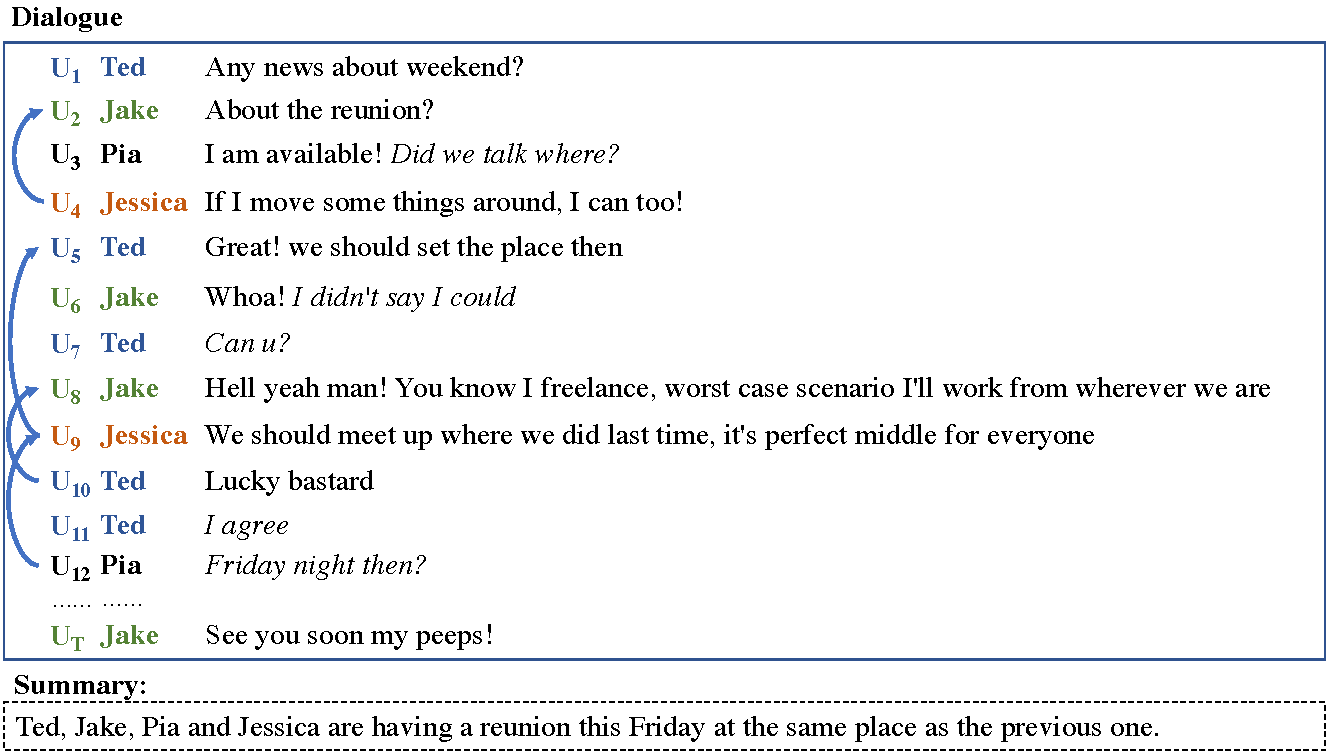
\includegraphics[scale=0.5]{fig/example.pdf}
	\caption{An example multi-party dialogue and its summary. The arrows represent unsequential dependencies between utterances. Elliptical sentences are in italic.}
	\label{fig:example}
\end{figure}

\textbf{Word Level - Language Style and Format:} 
Documents in previous well-researched summarization tasks are written from the third point of view, while dialogues consist of utterances expressed by different speakers in first person. Informal and colloquial expressions are common especially for recorded dialogues from speech, such as ``Whoa'' in $U_6$ and ``u'' representing ``you'' in $U_7$ from Figure~\ref{fig:example}.
Pronouns are frequently used to refer to events or persons mentioned in the dialogue history. Around 72\% of mentions in the conversation are {anaphoras} %pronouns
as stated in \citet{bai2021joint}. Meanwhile, the performance of coreference resolution models trained on normal text drops dramatically on dialogues~\cite{liu2021coreference}. It manifests the existence of language style differences between documents and dialogues, leading to difficulties in understanding the mappings between speakers and events in dialogues.


\textbf{Sentence/Utterance Level - Information Density:}
Document sentences are more self-contained with complete SVO (subject-verb-object) structures, while elliptical utterances are ubiquitous in dialogues, including $U_3$, $U_6$, $U_7$, $U_{11}$ and $U_{12}$.
Besides, the long dialogue can be summarized into a single summary sentence for the example in Figure~\ref{fig:example} as a result of back-and-forth questions and confirmations among speakers for communication purposes.
Question answerings, acknowledgments, and comments~\cite{asher2016discourse} are frequent discourse relations among utterances to narrow down speakers' information gaps and reach agreements.
In this way, dialogue utterances are highly content-dependent, and the information is scattered~\cite{zhang2021exploratory}, raising the difficulties for generating integral contents.

\textbf{Inter-sentence/utterance Level - Discourse structure:}
Articles tend to be well-structured, such as 
general-to-specific structure or deductive order. 
For example, the most important information 
in news summarization are always at the beginning of the document, resulting in a competitive performance of the simple Lead-$3$ baseline~\cite{nallapati2017, see2017get}. However, it is not the same for dialogue summarization. Both Lead-$3$ and Longest-$3$, i.e. $\{U1, U2, U3\}$ and $\{U4, U8, U9\}$ in Figure~\ref{fig:example}, get poor results in different dialogue scenarios~\cite{gliwa2019samsum,chen2021dialsumm,zhang2021emailsum}.
The dependencies among utterances are interleaved, shown by arrows in Figure~\ref{fig:example}, and discourse relations in dialogues are more flexible,
even with the correction of wrong information~\cite{asher2016discourse}. 
For example, 
Jake refused to be available for the reunion in $U_6$, but later agreed
in $U_8$.  As a result, it is more challenging to reason cross utterances for 
dialogue summarization than document summarization.

\textbf{Passage/Session Level - Topic boundaries:} Sentences under the same topic in documents are collected together in a paragraph or a section.
Previous works for extractive~\cite{xiao2019extractive} and abstractive summarization~\cite{cohan2018discourse} both took advantage of such features and made great progress. 
However, a dialogue is a stream of continuous 
utterances without boundaries, even for hours of discussion. The same topic may be discussed repeatedly 
with redundancies and new information, setting up obstacles for content 
selection in dialogue summarization.

%\JQ{it will be good to see the advantages of abstractive vs extractive approaches for dialogue summarization.}
%\JQ{add a little more about extractive methods, and explain why abstractive is more preferred especially in the case of dialogues.}
To better explain why abstractive approaches are more preferred than extractive ones for dialogues, we list the result of the best rule-based extractive baseline, i.e., Longest-$3$~\cite{gliwa2019samsum}, the oracle extractive result determined by Rouge-L Recall score between each summary sentence and dialogue utterances~\cite{chen2018fast}, and the generation by BART fine-tuned on SAMSum dataset~\cite{gliwa2019samsum} of the simple dialogue in Figure~\ref{fig:example} as follows:
\\
\begin{tabular}{|p{1.5cm}|p{\linewidth-2.3cm}|}
	\hline
	\textbf{Longest-$3$} & Jessica: If I move some things around, I can too! Jake: Hell yeah man! You know I freelance, worst case scenario I'll work from wherever we are Jessica: We should meet up where we did last time, it's perfect middle for everyone.\\
	\hline
	\textbf{Oracle} & Jake: Hell yeah man! You know I freelance, worst case scenario I'll work from wherever we are\\
	\hline
	\textbf{BART}& Ted, Pia, Jessica and Jake are going to meet up on Friday night. \\
	\hline
\end{tabular}
\\
We can see that the readability of generated summaries are poor for Longest-$3$ and Oracle due to the language style and format difference. The compression ratio of Longest-$3$ is apparently low while it still misses the involvement of Ted and Pia as a result of low information density of dialogues. Oracle is concise but much more information is missing. Meanwhile, the fine-tuned BART as an abstractive approach shows the favorable performance. Therefore, abstractive approaches becomes the mainstream in researches on dialogue summarization. In a word, dialogue summarization is an valuable research direction in summarization, where the modeling and understanding of dialogues are challenging compared with document summarization and abstractive approaches are especially preferred.
% despite some extractive summarization works~\cite{uma2022comparing,kano2020identifying,bokaei2016extractive}.
%@article{uma2022comparing,
%	title={Comparing Methods for Extractive Summarization of Call Centre Dialogue},
%	author={Uma, Alexandra N and Sityaev, Dmitry},
%	journal={arXiv preprint arXiv:2209.02472},
%	year={2022}
%}

%@inproceedings{kano2020identifying,
%	title={Identifying implicit quotes for unsupervised extractive summarization of conversations},
%	author={Kano, Ryuji and Miura, Yasuhide and Taniguchi, Tomoki and Ohkuma, Tomoko},
%	booktitle={Proceedings of the 1st Conference of the Asia-Pacific Chapter of the Association for Computational Linguistics and the 10th International Joint Conference on Natural Language Processing},
%	pages={291--302},
%	year={2020}
%}

%@article{bokaei2016extractive,
%	title={Extractive summarization of multi-party meetings through discourse segmentation},
%	author={Bokaei, Mohammad Hadi and Sameti, Hossein and Liu, Yang},
%	journal={Natural Language Engineering},
%	volume={22},
%	number={1},
%	pages={41--72},
%	year={2016},
%	publisher={Cambridge University Press}
%}


\subsection{Scenarios for Dialogue Summarization}\label{sec:scenarios}

Considering the source of dialogues and the purpose of doing summarization,
%\KZ{Rephrase this: dialogue sources and summary intentions}, 
we divide the application scenarios into two classes: \textbf{open-domain dialogue summarization (ODS)} and \textbf{task-oriented dialogue summarization (TDS)}. This taxonomy is similar to the one of dialogue systems~\cite{gao2020standard,chen2017survey}.
However, one should note that a pre-defined domain ontology for dialogues is 
not necessarily required for TDS, which is different from that in 
task-oriented dialogue systems.
The application scenarios investigated in previous papers 
are classified into these two classes as shown in Figure~\ref{fig:scenario}.

%\JQ{add citations}
Open-domain dialogue summarization is further divided into daily chat, 
drama conversation, debate \& comment. 
\textbf{Daily chat}~\cite{gliwa2019samsum,chen2021dialsumm} refers to the dialogues happening in our daily lives, 
such as making appointments, discussions between friends, etc. 
\textbf{Drama conversation}~\cite{rameshkumar2020storytelling,zhu2021mediasum,malykh2020sumtitles,chen2021summscreen} represents dialogues from soap operas, 
movies or TV shows, which are dramatized or fabricated with drama scripts 
behind them. Dialogues in these two classes are full of person names 
and events, resulting in narrative summaries about ``who did what''.
\textbf{Debate \& comment}~\cite{misra2015using,fabbri2021convosumm,chowdhury2019cqasumm} focuses more on question answering and 
discussions in online forums and arguments. These dialogues emphasize opinions or solutions to the given subject or questions.

Task-oriented dialogue summarization arises from application scenarios of different domains, which includes but is not limited to customer service, 
law, medical care and official issue.
\textbf{Customer service}~\cite{zou2021topic,feigenblat-etal-2021-tweetsumm-dialog,zhao2021todsum,liu2019automatic,chen2020jddc} refers to conversations between customers and service providers.
Customers start the conversation with their specific intents and agents are required to meet these requirements with the help of their in-domain databases, such as hotel reservations and express information consultation for online shopping. Dialogue summarization for this task is mainly to help service providers quickly go through solutions to users' questions for agent training and service evaluation. 
\textbf{Law}~\cite{fuzw20,duan2019legal,xi2020global} is dialogues related to legal service and 
criminal investigations. Dialogue summarization in this scenario alleviates the recording and summarizing workload 
for law enforcement or legal professionals. 
\textbf{Medical care}~\cite{joshi2020dr,song2020summarizing,song2020summarizing,zhang2021leveraging,liu2019topic} is dialogues between doctors and patients and medical dialogue summarization has some similarity to the research on electronic health records (EHR). Unlike the previous work focusing on mining useful information from EHR~\cite{yadav2018mining}, summarization is to extract useful information from the doctor-patient dialogue and generate an EHR-like or fluent summary for clinical decision-making or online search. It also aims to reduce the burden of domain experts.
\textbf{Official affair}~\cite{carletta2005ami,janin2003icsi,ulrich2008publicly,zhang2021emailsum} is conversations between colleagues for technical or teachers and students for academic issue discussion. They can be either in the format of meetings or e-mails, with summaries covering problems, solutions, and plans.


\begin{figure}
	\centering
	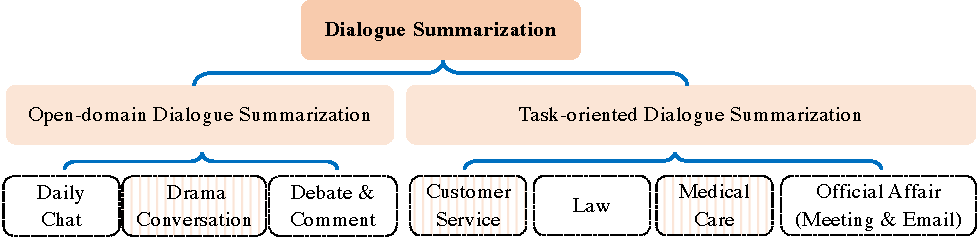
\includegraphics[scale=0.8]{fig/scenarios.pdf}
	\caption{The classification of dialogue summarization tasks with different application scenarios. Datasets proposed for evaluations under each scenario are in Section~\ref{sec:dataset}.}
	\label{fig:scenario}
\end{figure}


We compare and contrast ODS and TDS as follows.
\begin{itemize}
% functional role playing
\item Dialogues happen between \textbf{two or more speakers} both in ODS and TDS, whereas the \textbf{interpersonal relationship} and \textbf{functional relationship} among speakers are different. Generally, speakers in ODS are friends, neighbors, lovers, family members, and so on. 
They are equal either in the aspect of interpersonal relationships or functional relationships. For example, one can raise a question or answer others' questions in online forums~\cite{fabbri2021convosumm}.
In TDS, speakers have different official roles acting for corresponding responsibilities. For example, plaintiff, defendant, witness and judge in court debates~\cite{duan2019legal}, project manager, marketing expert, user interface designer and industrial designer in official meetings~\cite{carletta2005ami} are corresponding roles.
Among different dialogues, roles are the same and can be played by different speakers and a speaker's role is always unchanged for a service platform.
In a word, TDS pays more attention to functional roles while ODS focuses on speakers.


% covering topics
\item Multiple \textbf{topics} may be covered in the same dialogue session.
Topics in ODS are more diverse than in TDS. The summarization models are expected to deal with unlimited open-domain topics such as chitchat, sales, education, and climate at the same time~\cite{chen2021dialsumm}. 
However, topics in TDS are more concentrated and need more expertise for understanding.
Dialogues in TDS either focus on a single domain with more fine-grained topics, such as medical dialogues of different specialties,
or several pre-defined domains, such as restaurant, hotel, and transformation reservation.
Domain knowledge is significant for summarization, and it is divergent across sub-domains. For instance, expertise and medical knowledge are required in doctor-patient dialogues for generating accurate medical concepts~\cite{joshi2020dr} while specific knowledge bases for internal medicine and primary care are not the same.

%  inherent structure
\item The input dialogue for both ODS and TDS is made up of \textbf{a stream of utterance} as defined in Equation~\ref{eq:dialogue}. However, 
the \textbf{structure} of these two types of dialogues are different.
Open-domain dialogues often happen casually and freely while dialogues in TDS may have some inherent working procedures or writing formats. 
For example, the program manager in meetings usually masters the meeting progress~\cite{zhu2020end} implicitly with words such as ``okay, what about ...'', and communications by e-mails consist of semi-structured format including subjects, receivers, senders, and contents~\cite{zhang2021emailsum}. 

% special intentions for summaries
\item \textbf{Focuses of summaries} are distinct. Summaries for ODS in recent research are more like condensed narrative paraphrasing with different levels of granularity. An example is a synopsis from the Fandom wiki\footnote{\url{criticalrole.fandom.com}} maintained by fans for the Critical Role transcripts~\footnote{\url{github.com/RevanthRameshkumar/CRD3}}\cite{rameshkumar2020storytelling}, helping to quickly catch up with what is going on in the long and verbose dialogues. Differently, dialogues in TDS take place with strong intentions for solving problems. Summaries for such dialogues are expected to cover the user intents and corresponding solutions, such as medical summaries for clinical decision making~\cite{joshi2020dr} and customer service summaries for ticket booking~\cite{zhao2021todsum}. As a result, generating faithful content is extremely significant for TDS. %{faithfulness}
\end{itemize}

%\KZ{I feel that just dividing the dialogue summarization into ODS and TDS is a bit
%too coarse-grained. Later when you discuss the approaches, u need to associate
%each approaches with a certain characteristic/scenario of the task. It's more
%useful if u can use some refined characteristics of the task.}



\section{Technical Specification}
\label{sec:algo}

\begin{figure*}[th]
\centering
\epsfig{file=pic/SystemOverview2.eps,width=1.8\columnwidth}
\caption{System Overview}
\label{fig:sys}
\end{figure*}

Figure \ref{fig:sys} shows the block diagram of our system.
As the input of the system, the web page is first parsed by 
a HTML parser\cite{winista} to obtain a complete DOM representation.
Then the title classifier attempts to recognize the page title.
If it is a ``top-$k$ like'' title, 
the classifier outputs the list size (the number $k$) 
and a set of possible concepts mentioned in the title.
With the number $k$, the candidate picker extracts all lists of size $k$ 
from the page body as candidate lists. Only one of them will be the actual
list of interest. With the concept set, 
the top-$k$ ranker can score each candidate list and pick the best one 
as the ``top-$k$'' list.  Finally the content processor  
analyzes the list content and extracts the entity names and attributes. 
%and conceptualize the main entities in the list
%as well as their attributes, if any. 

\subsection{Title Classifier}
\label{sec:title}

The title of a web page (string enclosed in {\tt<title>} tag) helps us
identify a top-$k$ page.  There are several reasons for us to utilize
the page title to recognized a top-$k$ page.  First, for most cases,
page titles serve to introduce the topic of the main body.  Second,
while the page body may have varied and complex formats, top-$k$ page
titles have relatively similar structure.  Also, title analysis is
lightweight and efficient. If title analysis indicates that a page is
not a top-$k$ page, we chose to skip this page.
This is important if the system has to scale to billions of web pages.

\begin{figure}
\centering
\epsfig{file=pics/pageTitle2.eps,width=0.9\columnwidth}
\caption{A Sample Top-K Title}
\label{fig:title}
\end{figure}

%We now discuss what a top-$k$ title should look like.
%In general, a top-$k$ title represents the topic of a top-$k$ list.
Figure \ref{fig:title} shows a typical top-$k$ title.  Note that the title
may contain multiple segments, and usually only one segment describes
the topic or concept of the list.  In addition to the value of $k$
(e.g, 10) and the head concept (e.g, ``podcasts''), a top-$k$ title
may include some other elements, such as the ranking criteria (e.g,
``top'', ``most memorable'', etc.) and other modifiers (e.g, ``.net
Awards'' and ``2011'').

\ZZX{
Note that a web page with a top-$k$ title may not contain a top-$k$ list.
A typical case is shown in Figure \ref{fig:slideshow}. Here the top-$k$ list
is divided into multiple interlinked pages, instead of being on a single page.
Extracting such lists requires that all relevant pages are in
the corpus and are properly indexed which increases the cost of the solution
significantly. Base on our observations, such multi-page top-$k$ lists
account for about 5\% of the total number of top-$k$ lists on the web,
we therefore choose to ignore this type of pages in this paper.
%additional crawling (because it is not
%certain that each of the page is in the web corpus) and it is too
%costly given that we need to handle billions of pages already.
}

We build a classifier to recognize top-$k$ titles.
Specifically, we train a Conditional Random Field (CRF)
\cite{CRFLafferty} model from a labeled dataset of both
positive titles and negative titles (negative titles also contain a
number).  We use lexical features such as {\em word}, {\em lemma}, and
{\em POS tag}\cite{santorini1990part} to form the basic feature set.  The classifier also
returns additional information such as the list size $k$ and a set of
concepts (recorded by a knowledge base such as Probase)
which are mentioned in the title.
\ZZX{We prefer to optimize the classifier for higher recall rather
than precision at this step, because some false positives pages,
which cannot be recognized through titles alone,
can be easily filtered out by validating against other properties
during the List Extraction phase.}
%
%Since we have additional mechanisms that help us filter out
%false positives pages (i.e, pages that are wrongly recognized as
%top-$k$ pages), we optimize the classifier for getting higher recall.
%\KZ{What additional mechanism?}

\begin{figure}
\centering
\epsfig{file=pics/page4.eps,width=0.8\columnwidth}
\caption{A Slide-show Page Snapshot\cite{TopFootball}}
\label{fig:slideshow}
\end{figure}

\subsubsection{The CRF model}
We convert the problem of recognizing top-$k$ titles to the problem of
recognizing the number $k$ in a top-$k$ context. For example, in
Figure \ref{fig:title}, ``10'' is the $k$ in the top-$k$ context,
while ``2010'' is not a $k$ even though it is also a number.

We consider the ``$k$ recognition task'' as a sequence labeling
problem: Each word in the title is considered a token in a sequence,
and is either $k$ or {\em not k}.
%The \emph{TRUE} label means the corresponding token is the $k$, and
%the title sequence is therefore recognized as a top-$k$ title.
CRF is well suited to such tasks.
The main idea of CRF is to calculate the
conditional probability of the whole label sequence given the
observation sequence.  We define $X=(X_{1}, X_{2}, X_{3}, ..., X_{n})$ as
a word sequence of length $n$, and $Y=(Y_{1}, Y_{2}, Y_{3}, ..., Y_{n})$
as a label sequence, where $Y_{i} \in \{TRUE, FALSE\}$.  The CRF model
calculates the conditional distribution $P(Y|X)$, and then selects the
$Y$ that maximizes the probability.

We use the linear chain as the undirected statistical graphical model,
which is based on the assumption that each label $Y_{i}$ only depends on
its immediate neighbors ($Y_{i+1}$ and $Y_{i-1}$).
For linear chain CRF, the conditional probability can be calculated as:
\begin{equation*}
    P(Y|X)=\frac{1}{Z(x)}\exp(\sum_{i=1}^{n}\sum_{j=1}^{m}\lambda_{j}f_{j}(y_{i-1},y_{i},x,i))
\end{equation*}
where $Z(x)$ is a normalization factor, $f_{j}$ is one of the $m$
functions that describes a feature, and $\lambda_{j}$ is the feature
weight to be trained.
To build an effective CRF model, we need to collect training data and
design a feature set, which is discussed below.

%We can build an undirected graph $G(V,E)$ to represent each $Y_{i} \in Y$
%according to the independency relations
%(in other words, if $Y_{i}$ and $Y_{j}$ depend on each other,
%there is an edge connecting the two nodes).
%Therefore, the overall probability $P(Y|X)$ is equal to
%the product of the potential functions of all the maximal cliques in $G(V,E)$.


%For web titles,
%The structure of the label sequence can be an arbitrary undirected graph,
%which is different from hidden Markov model\cite{HMMBaum}.
%For title recognition, the graph of interest is linear chain.
%
%
%Since in normal NLP tasks (including the title classifier in our system), the graph of interest is usually a linear chain. We will focus on this model in the following discussion.
%
%, or CRF\cite{CRFLafferty},
%is a probabilistic model based on undirected graphs.
%
%
%We can convert the original problem of Title Classifier
%into to a $k$ recognition task,
%The task is to find a proper number word in title,
%of which the context conveys a top-$k$ topic.
%
%
%Therefore the task becomes a sequence segmentation problem:
%each word in the title is a token in sequence to be assigned


\subsubsection{Creating a training dataset}
\label{sec:titleDataSet}
Creating a large, high quality training dataset is costly. The
challenge mainly lies in collecting positive cases, as top-$k$ pages
are sparse on the web (approx. 1.4\textperthousand{} of total web pages, see
Section \ref{sec:eval}). Filtering out pages without a number in
the title narrows our candidates down, but the number of candidates
is still massive.
%Although narrowing down the target to those whose titles contain at
%least a number, it is still difficult to manually collect enough
%positive cases.
In our approach, we first tokenize the titles to add POS
tags, and then we adopt the following simple rules to identify
or create positive training samples.
\begin{itemize}
\item \textbf{``top CD''}: If a title contains the word ``top''
  followed by a number, it is likely to be top-$k$ title. For example,
  ``top 10 NBA players who could be successful general managers''.
\item \textbf{``top CD'' without ``top''}: A title which satisfies the
``top CD'' rule is still a top-$k$ title with the word ``top'' removed.
\item \textbf{``CD JJS''}: ``JJS'' stands for superlative adjectives.
  If a title contains a number followed by a superlative adjective, it
  is likely to be a top-$k$ title.  For example, ``20 tallest
  buildings in China''.
\item \textbf{``CD RBS JJ''}: ``RBS'' and ``JJ'' stand for superlative
  adverbs and adjectives, respectively.  If a title contains a number,
  followed by a superlative adverb, and followed by an adjective, it is
  likely to be a top-$k$ title.  For example, ``5 most expensive
  watches in the world''.
\end{itemize}

%We consider pages that satisfy any of the three rules above.  The
%three rules can only cover about 50\% of top-$k$ titles.  But in fact,
%it is unnecessary that the top-$k$ titles in the training dataset must
%be titles of real web pages: We can simply ``make up'' these titles,
%or create positive top-$k$ titles on our own.

% In fact, we can automatically generate ``top-$k$ like'' titles
% that satisfy none of the rules above from the ``top-$k$ like'' titles
% that satisfy the first rule, according to the following observation.
%We can directly build a classifier based on the three rules. About this rule-based classifier, there is good news and bad news.
%The good news is that the precision of the classifier is very high. The bad news is that there are still many ``top-$k$ like'' titles that do not satisfy the three rules, such as ``10 movies that you should not miss''. In fact, these rules can only cover half of all the ``top-$k$ like'' titles, in other words, the recall is only about 50\%.
%Since we put the recall performance of the title classifier in the first place, this rule-based approach is not completely qualified.
%But at least, these rules solve half of the problem, so now we can focus on the remaining ``top-$k$ like'' titles.

%The true reason that we have such a bottleneck is that we make an unnecessary assumption, that the titles in the training data set must be titles of real web pages. Instead of collecting titles of top-$k$ pages, we can just ``make up'' these titles, which is much easier.
%In fact, we can automatically generate ``top-$k$ like'' titles that satisfy none of the rules above from the ``top-$k$ like'' titles that satisfy the first rule, according to the following observation.

%In fact, we have the following observation: {\it For a title that
%  satisfies the rule ``top CD'', it will still be a top-$k$ title if
%  we remove the word ``top''.} For example, for the title ``top 10 NBA
%players who could be successful general managers'', we can delete
%``top'' to get ``10 NBA players who could be successful general
%managers'', which is still a top-$k$ title.  This is true for most
%cases, as ``top'' is the default criteria when making a top-$k$
%list.  With this method, we increase the number of positive
%cases.
% generate the $N$ positive cases in a full automatical manner:
% first we obtain $N/2$ titles using the ``top CD'' rule; then we remove
% the ``top'' in each title and get $N/2$ new titles.  Combined with $M$
% negative cases, we finally have a large enough training data set.

\subsubsection{Extracting features}
We now discuss how we extract features from a title.  As we see in
Figure \ref{fig:title}, a title may contain multiple segments, which
are separated by separators like ``-'' or ``$|$''.  Among these
segments, only the main segment (e.g, Segment 1 in Figure
\ref{fig:title}) gives us the topic of the page, while other
segments show additional information such as the name of the site,
which is not of interest. We therefore split the title and retain
only segments that contain a number.

Instead of extracting features from a title as a whole, we focus on a
fixed-size window centered around the number $k$ in the title. We argue
that the number $k$ serves as an anchor to a phrase that represents
a top-$k$ concept or topic.
For a window of large enough size $n$, the $n$-gram is
sufficient to make a correct judgement.  With this observation,
we transform the original task into the task of recognizing the
number $k$ with a proper context,
which is much easier and more suitable for CRF
learning.  % Last but not the least, if we use the whole sentence as the
% model pattern, we have to manually solve the number ambiguity if the
% title contains multiple numbers.  While for $n$-grams, we only label
% the center number word that satisfy the rule ``top CD'', so that we
% can do labeling automatically.
  % as ``TRUE'', otherwise ``FALSE''.
% Furthermore, since
% with Unlike other model pattern that use the whole sentences, our
% model pattern only pick a fixed-length context of a number word.
% \ref{tab:modelPattern}.


  %If we use the whole sentence as the model pattern,
  %  . Otherwise

%With the training data set, we would like to use the tool CRF++\cite{crfppHome} to generate the classifier model.
%Before we do that, we have to design the model pattern first. The model pattern is the input format for CRF++ to learn or test data,
%including used features, meaning of tokens, set of answer tags and so on. Figure \ref{fig:crfpp}(a) shows a sample model pattern.

%We use a model pattern as a $n$-gram centering on a number word.
Table \ref{tab:modelPattern} shows an example of feature extraction
with a window size $n=9$.  If there are not enough words before or
after the centered number, we just fill up the vacancies with the null
token. We select four features: \emph{word}, \emph{lemma},
\emph{POS tag} and \emph{concept}.  The {\it lemma} feature gives the original
form of the word.  For example, the lemma for ``podcasts'' is
``podcast''.  The {\it POS tag} feature indicates the part-of-speech
of a word.  The {\it concept} feature indicates whether the word
forms a string suffix of a concept in a knowledge base.
The $i$th bit of the concept feature value is set to 1 if the
$i$-gram that ends with the word is a concept.
  %, especially the first bit is the case for the word itself.
In Table \ref{tab:modelPattern}, the concept value for
``podcasts'' is 1, which means ``podcast'' is a concept.
For a phase ``Asia companies'', the concept value for
``companies'' is 3, because both ``companies'' and ``Asia companies''
are concepts from the knowledge base.


% Using the pattern above,
% we successfully trained a CRF model with the training data ,
% now we can build the outside title classifier.

\begin{table}
\centering
\caption{Feature extraction from a window of  size 9. (Vacancies are filled with the null token.)}
\begin{tabular}{|l|l|l|l|l|}
\hline
\textbf{word}    &\textbf{lemma}   &\textbf{POS}    &\textbf{concept}   &\textbf{tag} \\ \hline
.net        &net        &JJ	    &1  &FALSE\\
awards      &award      &NNS	&1  &FALSE\\
2011        &2011       &CD	    &0  &FALSE\\
top         &top        &JJ	    &1  &FALSE\\
10          &10	        &CD     &0  &TRUE\\
podcasts	&podcast    &NNS	&1  &FALSE\\
NULL        &NULL       &NULL	&NULL  &FALSE\\
NULL        &NULL       &NULL	&NULL  &FALSE\\
NULL        &NULL       &NULL	&NULL  &FALSE\\
\hline
\end{tabular}
\label{tab:modelPattern}
\end{table}

\subsubsection{Using the classifier}


\begin{figure}
\centering
\epsfig{file=pics/TitleClassifier.eps,width=0.9\columnwidth}
\caption{The Flow Chart of the Title Classifier}
\label{fig:titleClassifier}
\end{figure}

Figure \ref{fig:titleClassifier} shows how we use the classifier.  (1)
The preprocessor generates features.  (2) The classifier labels the
$n$-gram pattern as \emph{TRUE} or \emph{FALSE}.  (3) If it is
identified as a top-$k$ title, the postprocessor extracts additional
information from the title, which includes the value of $k$, the
ranking criterion, and
the concepts mentioned in the title.  For example, in this case, the
concepts include $\{``.net'',``awards'', ``podcasts''\}$. These
information is used in the subsequent list extraction process.
In addition, to extract optional information like time and location,
the title is further processed by Content Processor which will be discussed
later.
%
%Before the title splitter, we need to filter ill-formatted
%writing in the title and lowercase all the words.
%%in order to optimize the performance of Stanford Parser.
%
%The model will label the $n$-gram pattern with \emph{TRUE} or \emph{FALSE},
%just like the last column in Table \ref{tab:modelPattern}.
%A \emph{TRUE} means the corresponding word is a proper number $k$,
%thus the corresponding title is a ``top-$k$ like'' title.

%The model will attach an additional column to the input 9-gram as the answer tag. The answer tag is either ``TRUE'' or ``FALSE''.
%We are only interested in the 5th tag, which indicates whether this title is a ``top-$k$ like'' title.
%If the 5th tag is ``TRUE'', the input is then a ``top-$k$ like'' title.


%is  {``scientist'',``influential scientist'', ``today''}.

%In Subsection \ref{sec:evalTitle}, we make an experiment to test the performance of the title classifier.
%The result is satisfying: the precision is over 75\% while the recall is over 90\%. As a conclusion, the model-based classifier is qualified for our system.


%
%The goal of the classifier is to recognize ``top-$k$ like'' titles,
%the likely name of a top-$k$ page. In general,
%a ``top-$k$ like'' title represents the topic of top-$k$ list.
%Figure \ref{fig:title} shows a typical ``top-$k$ like'' title.
%Note that a ``top-$k$ like'' title may contain multiple segments, and
%usually only one segment describes the topic or concept of the list.

%Besides the features we mentioned in Subsection \ref{sec:intro}
%(concept and number $k$),
%a ``top-$k$ like'' title could include some other elements;
%also as a web page, it may contain multiple segments,
%among which only one segment is the main part.

%Therefore, the actual task for Title Classifier is
%trying to recognize a proper number k with proper context in the title.
%If no such k is found, we consider the title not a ``top-$k$ like'' title.

%In our implementation, we build our classifier using a supervised machine-learning method.

%We trained a Conditional Random Fields (CRF) \cite{CRFLafferty} model
%from 4000 negative titles (titles that contains a number but
%are not actually ``top-$k$ like'') and 2000 positives titles. The number $k$
%is especially important because it serves as an anchor to a phrase that
%represent a ``top-$k$ like'' concept or topic.
%We use \textit{word, lemma,} and \textit{POS tag} \cite{StanfordParser}
%as the basic feature set.

%Among these features, the number k is especially important for
%our system for the following reasons:
%\begin{enumerate}
%\item The number k is the common feature among all ``top-$k$ like'' titles,
%while other features may omit in some titles
%\item The number k is indispensible for following components in our system:
%we need to extract a list with exact k items.
%\item We can reduce our target page group to
%``those pages whose title contains at least one number''.
%\end{enumerate}

%Before we test an input title with the model we learned,
%%we need to tranfer it to the format that our model can recognize
%%(the same format for training data).
%%Thus
%the following preprocessing steps are needed:
%
%\begin{enumerate}
%\item \textit{Normalizer}:
%Fix some ill-formatted writting in the title and lowercase all the words.
%\item \textit{Title Splitter}:
%Split the title into segments by splitters such as ``|'' and ``-'',
%and select the longest one with a number as the main segment.
%\item \textit{Feature Generater}:
%Generate mentioned features for each word in the main segment.
%We use Standford Parser \cite{StanfordParser} to get the lemma and POS tag features.
%After this, we can get a table with words as rows and features as columns.
%\end{enumerate}
%
%After that, we can test the feature table of the input title.
%The model will label the number in the title with ``T'' or ``F'',
%where ``T'' means the whole title is ``top-$k$ like''.


%%% Local Variables:
%%% mode: latex
%%% TeX-master: "paper"
%%% End:


\section{Candidate Picker}
\label{sec:picker}
Given an HTML page body and the number $k$,
the candidate picker collects a set of lists as candidates.
Each list item is a text node in the page body.

We define a {\em tag path} of a node as a path from the root to this node
in the DOM tree.
Items in a ``top-$k$'' list usually have similar format and style,
and therefore they share an identical tag path.
For example, in Table \ref{tab:sampleoutput},
the tag path corresponding to the second column {\em Name} is
{\tt html/body/.../p/strong}.

Based on this observation, our algorithm runs in four steps:
First, we preprocess the DOM tree to normalize the content of text nodes
(remove non-printable characters and shorten continuous spaces, etc.).
Second, we prune the DOM tree by cutting subtrees that include ``blacklisted''
attributes such as ``sidebar'' and ``comment'', because these often indicate
they are not the main content of the page.
%so that we can get avoid of most adversitements and user comments.
Third, we compute the tag path for every node in the DOM tree of the
input page. Finally, we group nodes with an identical tag path into
one {\em equivalence class}, and we
select those equivalence classes which have exactly $k$ members as our
candidate lists.

The above algorithm, known as the {\em Default} algorithm, achieves good
recall, but may produce noise. To further improve the precision,
we introduce three additional pattern-based rules to filter the candidate lists:

\begin{enumerate}
\item \textit{Index}:
There exists an integer number in front of every list item, serving as
a rank or index: e.g., ``1.'',``2.'',``3.'', ..., the numbers are in sequence
and within the range of $[1, k]$.

\item \textit{Highlighting tag}:
The tag path of the candidate list contains at least one tag
among {\em <b>,<strong>,<h1-h6>} for highlighting purposes.

\item \textit{Table}:
The candidate list is shown in a table format.
\end{enumerate}

In this modified algorithm, a.k.a. {\em Def+Patt} algorithm,
only candidates that satisfy at least one of the rules above are
kept and output to the next step.
For example the ``top-$k$'' list in Figure \ref{fig:topscientists}
satisfies rules 1 and 2.



\subsection{Top-K Ranker}
\label{sec:ranker}

When there are multiple candidate lists,
we select only one of them as the {\em main list}.
Intuitively, the main list is the one that best matches the title.
In Subsubsection \ref{sec:title}, we extract a set of concepts from
the title, and one of them should be the central concept of the top-$k$ list.
Our key idea is that one or more items from the main list should be instances
of one of the concepts extracted from the title. For example, if the title
contains the concept ``scientist'', then the items of the main list should
be {\em instances} of the ``scientist'' concept. The Probase taxonomy provides
large number of concepts and their instances. 
For instance, ``scientist'' concept has 2054 instances in Probase.
%Considering the fact that Probase cannot cover all the instances and
%concepts in the world,
We calculate the score of each candidate list $L$ as:

\[Score(L)= \frac{1}{k} \sum_{n \in L} \frac{LMI(n)}{Len(n)}\]
where $LMI(n)$ is the word count of the longest matched
instance in the text of node $n$,
while $Len(n)$ means the word count of the entire text in node $n$.

If there is a tie in $score(L)$, we prefer the list with the largest
{\em visual area} in the page.
The visual area is estimated by calculating text area
of the candidate list:

\[Area(L)= \sum_{n \in L} (TextLength(n)\times FontSize(n)^2).\]

%After we know the main list, we can also get attribute lists that
%are interleaved with the main list.


\subsection{Content Processor}
The content processor takes as input a ``top-$k$'' list and
extracts the main entities as well
as their attributes.
%normalized and conceptualized ``top-k list'' to the output.
%It has two major tasks:
Sometimes the text within an HTML text node contains a structure itself, e.g.
``Hamlet By William Shakespear''. The content processor infers the structure of
the text \cite{Fisher08:dirttoshovels} by building a histogram for
all potential separator tokens such as ``By'', ``:'' and ``,'' from all the items
of the ``top-$k$'' list. If we identify a sharp spike in the histogram for a
particular token, then we successfully find a separator token, and we use that
token to separate the text into multiple fields.

It is useful provide names to the extracted attribute values. For example,
we want to infer ``name'', ``image'', and ``Wikipedia link'' as
attribute names from the list in Figure \ref{fig:topscientists}.
To do this, we conceptualize the extracted columns \cite{Song11:Conceptualize},
using Probase and a Bayesian model.
%who utilized Probase \cite{WuLWZ12:Probase} as knowledgebase and
%developed a short text understanding system based on Bayesian model.
In addition, for special columns like indexes, pictures and long paragraphs,
we apply specified rules to conceptualize them.




\section{Injecting Pre-processed Features} 
\label{sec:feature}
To pursue better dialogue understanding and reasoning, different features either designed by experts back on linguistic knowledge or engineered with observations are proposed to simulate the human comprehension process.
Recognizing these features is not only independent dialogue analysis 
tasks but also critical enablers for downstream applications. 
A subset of these features has been proved helpful for dialogue summarization by extracting from $D$ explicitly and injecting it into the vanilla model.
We group different features into two sub-categories by their scopes:
\begin{itemize}
	\item \textbf{Intra-utterance features} are features within an utterance or for an individual utterance.
	\item \textbf{Inter-utterance features} are features connecting or distinguishing multiple utterances.
\end{itemize}



\subsection{Intra-Utterance Features}

We divide the intra-utterance features into three groups: word-level, 
phrase-level or utterance-level.


\subsubsection{Word-level}
Word-level intra-utterance features include TF-IDF weights, Part-of-speech (POS) tags, and named entity tags.

The \textbf{TF-IDF weight} is a well-known statistical feature for each word, signifying its importance in the whole corpus. 
Term-frequency (TF) is the number of word occurrences in a dialogue or an utterance divided by the number of words. Inverse-document-frequency (IDF) refers to the logarithm of the number of dialogues or utterances divided by the number of them containing the word.
Each dialogue or utterance can be represented by a vocabulary-sized TF-IDF weight vector, where each element is the product of TF and IDF. 
In early work, \citet{murray2005extractive} used such utterance vectors as features for classifiers to find important utterances.
This feature is still prevalent in constructing better prompts for the summary generation with large language models~\cite{prodan2021prompt}.


\textbf{POS tags} and \textbf{named entity tags} are linguistic labels assigned for each word. POS tags represent grammatical properties, including nouns, verbs, adjectives, etc. Named entity tags belong to pre-defined categories such as person names, organizations, and locations. Both of them are easily labeled by well-known NLP packages such as NLTK and Spacy, 
and can be assigned to summaries in the training set~\cite{OyaMCN14,singla2017spoken}, to generate summary templates for abstractive text summarization without neural models. 
\citet{zhu2020end} trained two embedding matrices for both tags and concatenated them with word embeddings as part of the embedding layer for the model, i.e.
$x_i^t = [e_i^t;POS_i^t;ENT_i^t]$. 
$e_i^t$, $POS_i^t$, and $ENT_i^t$ are the word embedding, POS embedding, and named entity embedding for $x_i^t$, respectively. These features, which were also adopted by \citet{qi2021improving} in the same way, work for hierarchical models trained from scratch on this task and 
help with language understanding and entity recognition. 
However, the probing tests indicated that pre-trained 
language models have already captured both features well 
implicitly~\cite{tenney2018you}, and the two are no longer 
needed. 

\subsubsection{Phrase-level}
Intra-utterance features here have key phrases/words and negation scopes.
 
\textbf{Key phrases/words} emphasize salient 
n-grams in the original dialogue, which can help with the information scattering challenge and lead to more informative summaries. 
The definition of key phrases varies.
\citet{wu2021controllable} regarded the longest common sub-sequence (LCS) between each candidate phrase, extracted from $D$ first using a trained constituency parser, and $Y$ as key phrases. 
The LCSs are concatenated into a sketch, 
which is prefixed to $Y$ as a weakly 
supervised signal for the summary generation. 
Similarly, \citet{zou2021topic} proposed that words that appear both 
in $D$ and $Y$ are salient or informative topic words, i.e., another kind of keywords. 
They used an extension of the Neural Topic Model (NTM)~\cite{miao2017discovering} to learn the word-saliency correspondences. 
Then, input utterances are converted to topic representations by the saliency-aware NTM and further incorporated into Transformer Decoder layers for a better extractor-abstractor two-stage summarizer.
Differently, \citet{feng2021language} regarded unpredictable words by DialoGPT as keywords since they assumed that highly informative words could not be predicted. 
They appended all extracted keywords at the end of $X$ as inputs to the summarization model. 


The \textbf{negation scope} is also a set of consecutive words  
reflecting denied contents in utterances. \citet{chen2020multi} pointed out that negations are challenging for dialogues. With that in mind, \citet{khalifa2021bag} trained a Roberta model on CD-SCO dataset~\cite{morante2012sem} for negation scope prediction, which labels the beginning and end positions of sentences' negation scopes in $D$ with designated special tokens. Unfortunately, inputting such labeled $D$ to the model hurt the performance according to their experiment results. Negations are of great importance in task-oriented scenarios for generating accurate facts, such as realizing the patient's confirmation or negation of a symptom in a medical care conversation. \citet{joshi2020dr} proposed using an additional binary vector to label each $x_i$ based on a set of manually-curated negative unigrams, and to modify the cross-attention distribution. Besides, they extended the vocabulary with a special token `[NO]' and 
learned when to generate it by formulating the probability distribution over extended vocabulary, similarly to~\citet{see2017get}. The results showed reductions in coherency despite capturing negations.


\subsubsection{Utterance-level}
Speakers or roles, redundancies, user intents, and dialogue acts are utterance-level intra-utterance features. 
Domain knowledge is another kind of intra-utterance feature. It lies across phrase-level to utterance-level depending on specific circumstances. 

\textbf{Speaker} or \textbf{role} is a naturally provided ``label'' for each dialogue utterance. 
Since the general default input to models is the concatenation of all of 
the utterances into a sequence of tokens, each speaker or role token $s_t$ 
is encoded just like any other content token $w_i^t$~\cite{chen2020multi,feng2021language}. Thus, the speaker or role 
information is likely ignored or misunderstood, especially by language models pre-trained 
on common crawled texts. 
For a better utilization of speaker information, \citet{lei2021hierarchical} introduced Speaker-Aware Self-Attention made up of Self-Self Attention and Self-Others Attention, which only considered whether utterances were from the same speaker. This structured feature is also 
adopted in~\cite{lei2021finer}.
In addition, the number of speakers is used as a feature for 
finding similar dialogues in the training set by \citet{prodan2021prompt}.
In TDS, the number of roles is always fixed in a specific scenario, although the speakers are various among dialogue sessions.
\cite{yang2022tanet} modified the input with template ``\{\textit{speaker}\} of role \{\textit{role}\} said: \{\textit{utterance}\}''.
Other previous work only focuses on modeling roles, reflecting functional information bias in utterances. 
The cheapest way is to represent each role with a dense vector $r_t$ which is either obtained by randomly initialized trainable vectors~\cite{zhu2020end,duan2019legal,qi2021improving,gan2021inspectional,asi2022end} or a small trainable neural network~\cite{song2020summarizing}. This vector is further concatenated, summed up, or fused by non-linear layers with input embeddings $e_i^t$ or utterance-level representations $h_t^u$ in summarization models. 
There are also works that capture such features by different sets of model parameters for different roles~\cite{zou2021topic,zhang2020unsupervised,yuan2019scaffolds}. More complicated methods that regard speakers or roles as graph nodes beyond the utterance-level are in \secref{sec:graphs}.


Since dialogue utterances are mixed with backchanneling or repetitive confirmations~\cite{sacks1978simplest}, \textbf{redundancy} is also a significant 
feature where each utterance is either preserved or removed. 
\citet{murray2005extractive} and \citet{zechner2002automatic} regarded 
utterances similar to the previous ones as redundant by calculating 
the cosine similarity between two sentence vectors 
computed using TF-IDF features. {Then, the remaining utterances can be regarded as a summary}.
Different from previous work calculating similarities between individual utterances,
\citet{feng2021language} brought the context into consideration which calculated similarities on the dialogue level.
Utterance representations $h_t^u$ are collected by inputting the whole dialogue into DialoGPT~\cite{zhang2020dialogpt}. 
Then, they assume that if adding an utterance $u_{t+1}$ to the 
previous history $\{u_1, ..., u_t\}$ doesn't result in a big difference 
between the context representation $h_t^u$ and $h_{t+1}^u$, 
$u_{t+1}$ will be regarded as a redundant utterance. 
Such features will be added as part of the dialogue input with special tokens. 
\citet{wu2021controllable} regarded non-factual utterances 
such as chit-chats and greetings as redundancies, and removed them by a sentence compression method with neural content selection for their summary sketch construction.

Another group of utterance-level features is matching each utterance with 
a label from a pre-defined multi-label set. \citet{wu2021controllable} defined 
a list of interrogative pronoun category to encode the \textbf{user intent}, including \textit{WHY}, \textit{WHAT}, \textit{WHERE}, 
\textit{WHEN}, \textit{CONFIRM} and \textit{ABSTAIN}. 
Each utterance is labeled by a few heuristics and these user intents are combined with the keywords and redundancies mentioned above as a sketch prefixed to the summary output.
This definition is different from the so-called user intent in task-oriented dialogue systems, while the latter can be used for TDS and will be discussed in domain ontologies in \secref{sec:graphs}.

A more widely-accepted label set is \textbf{dialogue act}, which is defined as the functional unit used by speakers to change the context~\cite{bunt1994context} and has been used for different goals~\cite{kumar2018dialogue, oraby2017may}. The whole dialogue act taxonomy, including dialogue assess, inform, offer, etc., is tailored for different scenarios. For example, only 15 kinds of dialogue are labeled in the meeting summarization corpus AMI~\cite{carletta2005ami} 
while the total number of categories is 42~\cite{stolcke2000dialogue}. \citet{goo2018abstractive} explicitly modeled the relationships between dialogue acts 
and the summary by training the dialogue act labeling task and 
abstractive summarization task jointly. 
\citet{di2020da} further added the dialogue act information as a contextualized 
weight to $h_t^u$. These labels are required from human annotators. 

\textbf{Commonsense knowledge} generated by widely-used generative commonsense model PARA-COMET~\cite{gabriel2021paragraph} is considered in~\cite{kim2022mind}. PARA-COMET takes dialogue history with the target utterance or a summary sentence as input and outputs short phrases for each of the 5 relation types, which are strongly correlated with speakers' intentions and the hidden knowledge, such as ``XINTENT'' and ``XREACT''. The generated knowledge is concatenated with each utterance as input and is used as an additional generation target in a dual-decoder setting.

In addition, \textbf{domain knowledge} plays an important role in TDS. 
\citet{koay2020meet} showed that the existence of 
terms affects summarization performance substantially. 
Such knowledge is considered as intra-utterance features in previous work.
\citet{joshi2020dr} leveraged a compendium of medical concepts for 
medical conversation summarization. They incorporated domain knowledge at 
the phrase level by simply encoding the presence of medical concepts, which 
are both in the source and the reference. The corresponding one-hot vectors 
affect the attention distribution by the weighted sum with contextualized 
hidden states $H$ for each word only during training, like the teacher forcing strategy.
\citet{gan2021inspectional} defined a number of domain aspects, and labeled text spans manually in $D$ and $S$. Auxiliary classification tasks of these aspects help generate more readable summaries covering important in-domain contents. 
Differently, \citet{duan2019legal} incorporated their legal 
knowledge for each utterance. This is because their legal knowledge graph 
(LKG) depicts the legal judge requirements for different cases rather than a dictionary to look up, and each node represents a judicial factor 
requiring semantic analysis beyond the word level. A series of graph 
knowledge mining approaches were adopted to seek relevant knowledge w.r.t. 
each utterance $u_t$, and the legal knowledge embedding was added 
to the sentence embedding $h_t^u$ for further encoding.
 

\subsection{Inter-Utterance Features}\label{sec:interutt}

As dialogue utterances are highly dependent, information transitions among utterances are of great importance for dialogue context understanding. 
Multiple inter-utterance features show up for more efficient and 
effective dialogue summarization, which can be categorized into 
two sub-categories:
\begin{itemize}
	\item \textbf{Partitions} refer to extracting or segmenting the whole dialogue into relatively independent partitions. Information within each partition is more concentrated with fewer distractions for the summary generation. Meanwhile, these features reduce the requirements on GPU memory with shorter input lengths, which are especially preferred for long dialogue summarization.
	\item \textbf{Graphs} refer to extracting key information and relations from utterances to construct graphs, serving as a complement to the dialogue. These features are designed to help the summarization model understand the inherent dialogue structure.
\end{itemize}


\subsubsection{Partitions} 

There are two types of partitions.
One is to cut the dialogue into a sequence of $K$ consecutive segments $\{S_k|_{k=1}^K\}$ with or without overlaps, i.e., $|D|\leq|S_1| + ... + |S_K|$, where $|\cdot|$ counts the number of utterances. Representative features under this category are as follows.


\textbf{Topic transition} is important for dialogues where speakers turn to focus on different topics. Consecutive utterances that focus on the same topic constitute a topic segment, which should meet three criteria\cite{arguello2006topic}, including being reproducible, not relying heavily on task-related knowledge,  and being grounded in discourse structure.
Some previous works annotate this feature when constructing datasets such as \citet{carletta2005ami} and \citet{janin2003icsi}. 
\citet{di2020da} took advantage of such labeled information during decoding.
Others collected such features by rules or algorithms.
\citet{asi2022end} adopted the text segmentation idea from~\citet{alemi2015text} and broke the long dialogue into semantically coherent segments by word embeddings.
\citet{liu2019topic} regarded different symptoms as different topics in medical dialogues and detected the boundaries by heuristics.
To alleviate human annotation burdens, unsupervised topic segmentation methods are adopted. \citet{chen2020multi} used the classic segmentation algorithm C99~\cite{choi2000advances} based on inter-utterance similarities, where utterance representations were encoded by Sentence-BERT~\cite{reimers2019sentence}. \citet{feng2021language} regarded sentences that are difficult to be generated based on the dialogue context to be the starting point of a new topic. Thus, sentences with the highest losses calculated based on DialoGPT are marked.
However, the window size and std coefficient for C99 algorithm in %~\cite{choi2000advances} 
\citet{chen2020multi} and percentage of unpredictable utterances in \citet{feng2021language} are still hyper-parameters that need assigning by humans.
Among these works, some models use topic transitions as prior knowledge and input to summarisation models. They either add special tokens to dialogue inputs~\cite{chen2020multi,feng2021language}, add interval segment embeddings, such as $\{t_a, t_a, t_b, t_b, t_b, t_a,...\}$ for each utterance~\cite{qi2021improving}, or guide the model on learning segment-level topic representations $h_k^s$ based on utterance representations $h_t^u$~\cite{zheng2020abstractive}.
Others adjust their RNN-based models to predict topic segmentation first and do summarization based on the predicted segments~\cite{liu2019topic,li2019keep}, either with or without using additional supervised topic labels for computing the segmentation training loss. 

Multi-view~\cite{chen2020multi} describes \textbf{conversation stages}~\cite{althoff2016large} from a conversation progression perspective. They assumed that each dialogue contained $4$ hidden stages, which were interpreted as ``openings$\rightarrow$intentions$\rightarrow$discussions$\rightarrow$conclusions'', and annotated with an HMM conversation model. In their approach, both the preceding topic view and such stage view are labeled on dialogues with a separating token ``|'', encoded with two encoders sharing parameters and guided the Transformer decoder in BART with additional multi-view attention layers. 

There also exists a simple \textbf{sliding-window} based approach that regards window-sized consecutive utterances as a snippet and collects snippets with different stride sizes.
On the one hand, it can be used to deal with long dialogues. Sub-summaries are generated for each snippet and merged to get the final summary.
Most works regarded the window size and the stride size as two constants~\cite{koay2021sliding,liu2021topic,zhang2021leveraging,zhang2021summ},
while \citet{liu2021dynamic} adopted a dynamic stride size which predicts the stride size by generating the last covered utterance at the end of $Y'$.
\citet{koay2021sliding} generated abstractive summaries for each snippet by news summarization models as a coarse stage for finding the salient information.
On the other hand, pairs of (snippet, sub-summary) are augmented data for training better summarization models.
By calculating Rouge scores between reference sentences and snippets, 
the top-scored snippet is paired with the corresponding sentence~\cite{liu2021topic, zhang2021summ}.
Alternatively, multiple top-scored snippets can be merged as the corresponding input to the sentence~\cite{zhang2021leveraging} for the sub-summary generation. 
However, the gap between training and testing is that we don't know the oracle snippets since there is no reference summary during testing.
Therefore, each snippet was also considered to be paired with the whole summary~\cite{zhang2021leveraging,zhang2021summ}, but it leads to hallucination problems.
These constructed pairs can also be used with an auxiliary training objective~\cite{liu2021topic}, or as pseudo datasets for hierarchical summarization~\footnote{Hierarchical summarization means we do summarization, again and again, using the previously generated summaries as input to get more concise output. These models either share parameters~\cite{li2021hierarchical} or not~\cite{zhang2021leveraging,zhang2021summ} in each summarization loop.}.



The other is to \textbf{cluster utterances} or \textbf{extract utterances} into a single part or multiple parts $\{P_l|_{l=1}^{K'}\}$. In this way, outlier utterances or unextracted utterances will be discarded, i.e., $|D|>|P_1| + ... + |P_K'|$. Then, the abstractive summarization model is trained between the partitions and the reference summary. The whole process can be regarded as variants under the extractor-abstractor framework for document summarization~\cite{chen2018fast,liu2021keyword}. 

\citet{zou2021unsupervised} proposed to select topic utterances according to 
centrality and diversity\footnote{Centrality reflects the center of utterance clusters in the representation space. Diversity emphasizes diverse topics among selected utterances.} in an unsupervised manner. Each utterance with its surrounding utterances in a window size forms a topic segment.
\citet{zhong2021qmsum} extracted relevant spans given the query with the Locator model which is initialized by Pointer Network~\cite{vinyals2015pointer} or a hierarchical ranking-based model. 
Cluster2Sent by~\citet{krishna2021generating} extracted important utterances, clustered related utterances together and generated one summary sentence per cluster, resulting in semi-structured summaries suitable for clinical conversations. 
\citet{banerjee2015generating} and \citet{shang2018unsupervised} followed a similar procedure, i.e., (segmentation, extraction,  summarization) and (clustering, summarization) respectively.
The oracle spans are required to be labeled for supervised training of extractors or classifiers for most approaches, except that \citet{shang2018unsupervised} used K-means for utterance clustering in an unsupervised manner.
Generally, the partitions are concatenated as the input to summarization models~\cite{zhong2021qmsum}, or the generated summary of each segment is concatenated or ranked to form the final $\hat{Y}$~\cite{zou2021unsupervised,banerjee2015generating}.



\subsubsection{Graphs} 
\label{sec:graphs}

The intuition for constructing graphs is attributed to the divergent structure between dialogues and documents introduced in \secref{sec:divergence}. To capture the semantics among complicated and flexible utterances, a number of works constructed different types of graphs based on linguistic theories or observations and demonstrated improvements empirically. We group these graphs into three categories according to the type of 
nodes, i.e., being either a word, a phrase or an utterance. 

\textit{Word-level graphs} focus on finding the central words buried in the whole dialogue. Some works~\cite{OyaMCN14,banerjee2015generating,shang2018unsupervised,park2022unsupervised} parsed utterances together with or without summary templates using the Standford or NLTK packages. Words in the same form and the same POS tag or synonyms according to WordNet~\cite{MehdadCTN13} are regarded as a single node. The natural flow of text, parsed dependency relations and relations in WordNet are adopted to connect nodes, resulting in a directed \textbf{word graph}. It is used for unsupervised sentence compression by selecting paths covering nodes with high in-degree and out-degree without language models.

%Complex interactions within dialogues always make it hard for humans and models to associate speakers with correct events. At the same time, different surface forms of the same event and frequent coreferences increase the difficulty for the model to generate faithful summaries. 
The purpose for \textit{phrase-level graphs} is mainly to emphasize relations between important phrases.
\citet{liu2021coreference} and \citet{liu2021controllable} transferred document coreference resolution models~\cite{joshi2020spanbert,lee2018higher} to dialogues,  applied data post-processing with human-designed rules and finally constructed \textbf{coreference graphs} for dialogues. The nodes are mainly person names and pronouns, and the edges connect nodes belonging to the same mention cluster.
Based on the coreference results, \citet{chen2021structure} took advantage of information extraction system~\cite{angeli2015leveraging} and constructed an \textbf{action graph} with "WHO-DOING-WHAT" triples. 
\citet{zhao2021give} manually defined an undirected \textbf{semantic slot graph} based on NER and POS Tagging focusing on entities, verbs, and adjectives in texts, i.e., slot values. Edges in this graph represent the existence of dependency between slot values collected by a dependency parser tool.
More strictly defined ``domain-intent-slot-value'' tuples based on structured \textbf{domain ontologies} are marked in advance~\cite{yuan2019scaffolds,zhao2021todsum}. It is different from domain to domain, such as ``food, area'' slots 
for ``restaurant'' and ``leaveAt, arriveBy'' slot for ``taxi'' labeled in 
the MultiMOZ dataset~\cite{eric2019multiwoz}.
Ontologies in the medical domains containing clinical guidelines in 
``subject-predicate-object'' triples were introduced in~\citet{molennar2020healthcare}. Triples are extracted from $D$ and matched with the ontology to construct a patient medical graph for report generation.
Moreover, external commonsense \textbf{knowledge graphs}, 
such as ConceptNet~\cite{speer2012representing}, have been adopted to find the relations among speaker nodes, utterance nodes and knowledge nodes~\cite{feng2021incorporating}. 
%Their undirected graph use ``speaker-by'' edges connecting speaker nodes and utterance nodes and ``know-by'' edges connecting utterance nodes and knowledge nodes.



\textit{Utterance-level graphs} considering the relationship among utterances have been explored mainly in five ways. 
One is \textbf{discourse graph} mainly based on the SDRT theory~\cite{asher2003logics} which models the relationship between elementary discourse units (EDUs) with 16 types of relations for dialogues. Both \citet{chen2021structure} and \citet{feng2020dialogue} adopted this theory and regarded each utterance as an EDU. They labeled the dialogue based on a discourse parsing model~\cite{shi2019deep}. 
The former work used a directed discourse graph with utterances as nodes and discourse relations as edges.
Differently, the latter one transformed the directed discourse graph with the Levi graph transformation where both EDUs and relations are nodes in the graph with two types of edges, including default and reverse.  Self edges and global edges were also introduced to aggregate information in different levels of granularity.
\citet{ganesh2019restructuring} designed a set of discourse labels themselves and trained a simple CRF-based model for discourse labeling. Unfortunately, they haven't released the details so far.
\textbf{Dependency graph} can be regarded as a simplification of discourse graph since it only focuses on the ``reply-to'' relation among utterances.
The tree structure of a conversation is a kind of it and is adopted in~\cite{yang2022tanet} by modifying the self-attention into thread-aware attention which considers the distance between two utterances, and also proposing a thread prediction task to predict the historical utterances in the same thread for some sampled utterances.
Another one is \textbf{argument graph}~\cite{stede2016parallel} for identifying argumentative units, including claims and premises and constructing a structured representation. \citet{fabbri2021convosumm} did argument extraction with pretrained models~\cite{chakrabarty2019ampersand} and connected all of the arguments into a tree structure for each conversation by relationship type classification~\cite{mirko2020towards}. Such a graph not only helps to reason between arguments but also eliminates unnecessary content in dialogues. Similarly, \textbf{entailment graph}~\cite{MehdadCTN13} is used to identify important contents by entailment relations between utterances.
The fifth is \textbf{topic graph}. Usually, we regard the topic structure in dialogues as a linear structure as discussed above, but it can be hierarchical with subtopics~\cite{carletta2005ami, janin2003icsi} or non-linear structures since the same topic may be discussed back and forth~\cite{kim2019dynamic}.
\citet{lei2021finer} used ConceptNet to find the related words that indicate the connections among utterances under the same topic, capturing more flexible topic structures.


The graphs above are used in three ways. One is to convert the original dialogue into a narrative similar to documents by linearizing graphs and inputting to the basic summarization models~\cite{fabbri2021convosumm,ganesh2019restructuring}.
Second is to bring graph neural layers, such as Graph Attention Network~\cite{velivckovic2018graph} and Graph Convolutional Networks~\cite{kipf2016semi}. Such graph neural layer can be solely used as the encoder~\cite{feng2021incorporating}. It can also cooperate with the Transformer-based encoder-decoder models, either based on the encoder hidden states or injected into the Transformer layer in encoder~\cite{liu2021coreference} or decoder~\cite{chen2021structure}.
The rest modify attention heads in Transformer with constructed graphs from a model pruning perspective. \citet{liu2021coreference} replace attention heads containing the most coreference information with their coreference graph, while \citet{liu2023picking} replace underused heads with a similar graph.





\subsection{Multi-modal Features}

Humans live and communicate in a multi-modal world. As a result, multi-modal dialogue summarization is naturally expected. Even for virtual dialogues from TV shows or movies, character actions and environments in videos are important sources for humans to generate meaningful summaries. However, due to the difficulties of collecting multi-modal data in real life and the limited multi-modal datasets, this area remains to be researched. 
\textbf{Prosodic features} gained attention in early speech-related works.
\citet{murray2005extractive} collected the mean and standard deviation of the fundamental frequency, energy and duration features based on speech. %The features are collected at the word level and then averaged over the utterance.
With the marvelous automatic speech recognition (ASR) models, most works later only focused on transcripts and ignored such multi-modal features.
Besides, \textbf{visual focus of 
attention} {(VFOA)} feature from the meeting summarization scenarios 
has been introduced to highlight the importance of utterances~\cite{li2019keep}. 
It represents the interactions among speakers reflected by the focusing target that each participant looks at in every timestamp. They assumed that the longer a speaker was paid attention to by others, his or her utterance would be more important. Such orientation feature was converted into a vector by their VFOA detector framework and further concatenated to the utterance representations. 

\subsection{Summary and Opinions}

\begin{figure}
	\centering
	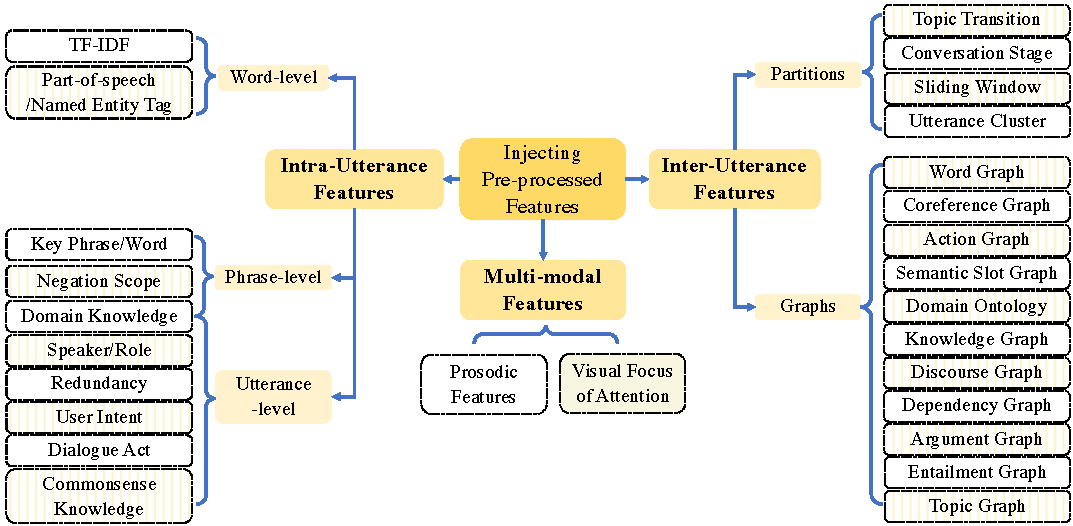
\includegraphics[scale=0.65]{fig/approach-feature.pdf}
	\caption{A summary of all features.}
	\label{fig:app-feature}
\end{figure}
The above features are summarized in 
Fig.~\ref{fig:app-feature} and mainly {injected into vanilla models} 
in three ways: 

\begin{itemize}
\item \textbf{Manipulating the input and output} by adding annotations or data reformulation. The former one adds additional tokens to the dialogue or summary to highlight the features, such as topic transition marks in the dialogue~\cite{chen2020multi} and key phrase prefixes of the summary~\cite{wu2021controllable}. This is suitable for features linearly buried in the texts. For the hierarchical or more complicated structures, researchers tend to reformulate the dialogue into different segments, especially for long dialogues~\cite{zhong2021qmsum,banerjee2015generating,shang2018unsupervised} or reordering utterances with graph features. For example,  \citet{fabbri2021convosumm} linearized the argument graph following a depth-first approach to fine-tune sequence-to-sequence models for summarization, and \citet{zhao2021todsum} linearized the dialogue states, i.e., slot-related labels, as a complement to $D$ with a bi-encoder model.



\item \textbf{Modifying the model architecture or hidden states} for learning inductive bias on known features. Embedding layers are always modified for word-level or phrase-level features indicating the binary or multi-class classification properties, including the POS embeddings in~\cite{zhu2020end} and medical concept embedding in~\cite{joshi2020dr}. Modifications on self-attentions and cross-attentions are used to merge multiple features and are also preferable to graph features. For instance, \citet{chen2020multi} modified the cross-attention layer for balancing and fusing hidden states of two kinds of labeled input from double encoders. \citet{lei2021hierarchical} changed the self-attention layer in the encoder with two speaker-aware attentions to highlight the information flow within the same speaker or among speakers. Different graph neural layers~\cite{feng2021incorporating,liu2021coreference,chen2021structure} are also introduced for capturing graph features.


\item \textbf{Adding additional training targets} means that features are regarded as a supervision output during training under multi-task learning and are ignored during inference. For example, \citet{goo2018abstractive}, \citet{li2019keep}, \citet{kim2022mind} used an additional decoder for dialogue act labeling, topic segmenting and commonsense knowledge generation, respectively.
\citet{yuan2019scaffolds} incorporated domain features by formulating domain classification as a multi-label binary classification problem for the whole $D$. All of them use utterance-level features to learn better encoder representations, which will lead to a high-quality summary.

\end{itemize}

The advantages and disadvantages of injecting pre-processed features are as follows:
\begin{itemize}
    \item[\Checkmark] Injecting pre-processed features as the mainstream research direction for dialogue summarization significantly improves the results compared with the basic summarization model. Features including negation scope, speaker/role, coreference graph, action graph and semantic slot graph pay more attention to generating consistent summaries, while most of the other features help to select valuable information for summarization.
    \item[\Checkmark] Such explicitly incorporated features are more interpretable to humans and can be manipulated for more controllable summaries. Different features can be selected and combined to promote the model performance in specific application scenarios.
        \item[\Checkmark] Features collected by labelers on other dialogue understanding tasks capture the essence of these tasks and also establish connections with various aspects of dialogue analysis.  Therefore, leveraging such features is a good way to alleviate the human labeling burden.
	\item[\XSolidBrush] Features are not transferable in different scenarios and some features are not compatible with each other, thus feature engineering is shown to be important.
	\item[\XSolidBrush] Labelers trained with other datasets are always out-of-domain compared to the targeting dialogue summarization scenario. Hyper-parameters introduced in labeling algorithms with these labelers need try and error for the domain transfer. 
	\item[\XSolidBrush] Error propagation exists in these dialogue summarization approaches. Incorrect features hinder the understanding of dialogues and lead to poor summaries. 
\end{itemize}
\section{Designing Self-supervised Tasks}
\label{sec:designselftasks}

To alleviate human labor and avoid error propagation, self-supervised 
tasks emerged, which leverage dialogue-summary pairs without additional 
labels.  We divide such tasks into three sub-categories:
\begin{itemize}
	\item \textbf{Denoising tasks} are designed for eliminating noises 
in the input or penalizing negatives.
	\item \textbf{Masking and recovering tasks} mean that parts of the input are masked and the masked tokens are required to be predicted.
	\item \textbf{Dialogue tasks} refer to response selection and generation for better dialogue understanding.
\end{itemize}


\subsection{Denoising Tasks}

Denoising tasks focus on adding
noises to the dialogue input or output and aims at generating concise summaries by filtering out the noisy information, resulting in more robust dialogue 
summarization models.
\citet{zou2021unsupervised} used the original dialogue as output and trained a denoising auto-encoder which is capable of doing content compression for unsupervised dialogue summarization.
Noising operations, which include fragment insertion, utterance replacement, and
content retention, are applied together on each sample.
For a utterance $u_t$ in $D$, \textbf{fragment insertion} means that randomly sampled 
word spans from $u_t$ is inserted to $u_t$ for lengthening the original 
sequence.
\textbf{Utterance replacement} is that $u_t$ is replaced by another utterance $u_{t'}$ in $D$ and \textbf{content retention} means that $u_t$ is unchanged. 
\citet{chen2021simple} augmented dialogue data by swapping, deletion, insertion 
and substitution on utterance level and used the corresponding summary as 
the output, resulting in more various dialogue inputs for training the summarization model. 
\textbf{Swapping} and \textbf{deletion} aim to perturb discourse relations by randomly swapping two utterances in $D$ or deleting some utterances.
\textbf{Insertion} includes inserting repeated utterances that are chosen from $D$ randomly and inserting utterances with specific dialogue acts such as self-talk or hedge from a pre-extracted set, mimicking interruptions in natural dialogues.
\textbf{Substitution} replaces the chosen utterances in $D$ by utterances generated with a variant of text infilling task adopted in the BART pre-training process.
Only one operation is adopted to noise $D$ at a time, and these operations pay more attention to dialogue characteristics, such as the structure and context information.


This kind of task can be extended to learn beyond the denoising ability when 
combined with contrastive learning or classification tasks on positive and negative data. 
Contrastive learning trains the model to maximize 
the distance between positive data and negative data for learning more informative semantic representations, which extends the classification's ability on generation tasks.
\citet{liu2021topic} 
proposed {coherence detection} and {sub-summary generation} 
for implicitly modeling the topic change and handling information scattering 
problems. They cut the dialogue into snippets by sliding windows and 
separated the long summary into sentences as a first step.
\textbf{Coherence detection} is to train the encoder to distinguish 
a snippet with shuffled utterances from the original ordered one.
\textbf{Designated sub-summary generation} is to train the model to generate more related 
summaries by constructing negative samples with unpaired dialogue 
snippets and sub-summaries, where the positive pair is obtained 
by finding the snippet with the highest Rouge-2 recall for each sub-summary.
\citet{tang2021confit} also designated summaries where negative summaries are constructed for different error types, such as swapping the nouns for wrong reference and object errors, swapping verbs for circumstance errors and tense and modality errors, etc. Positive summaries are collected by back translation. The distance of decoder representations measures the contrastive loss.
They also considered the \textbf{token identification} task to identify whether two tokens belong to the same speaker based on their encoder representations.
\citet{zhao2021give} made improvements by \textbf{perturbing hidden representations} of 
the target summary for alleviating the exposure bias following~\citet{lee2020contrastive}, which is useful for conditional generation tasks.

\subsection{Masking and Recovering Tasks} 

Masking and recovering tasks 
are commonly used in pre-training for better language modeling by recovering the original dialogue and 
bear some resemblance to the noising operations. The main difference is that these tasks try to recover the original text given the corrupted one.
It can be divided into 
work-level and sentence-level by the granularity of masked contents.
Word-level masks for \textbf{pronouns}~\cite{khalifa2021bag}, \textbf{entities}~\cite{liu2022entity,khalifa2021bag}, 
\textbf{high-content tokens}~\cite{khalifa2021bag}, 
\textbf{roles}~\cite{qi2021improving} and \textbf{speakers}~\cite{zhong2021dialoglm} are 
considered in previous work, for a better understanding of the complicated speaker 
characteristics and capturing salient information. Words masked 
in \citet{khalifa2021bag}'s work was determined by POS tagger, 
named entity recognition or simple TF-IDF features. Although the lexical 
features and statistical features have been captured by pre-trained models 
for different words as mentioned in \secref{sec:feature}, predicting 
the specific content words under these features reversely given the dialogue context is still challenging and helpful to dialogue context modeling especially with models pre-trained on general text.
Utterance-level masking objective inspired by \textbf{Gap Sentence Prediction}~\cite{zhang2020pegasus} is adopted by~\citet{qi2021improving}. Key sentence selection from dialogues is done by a graph-based sorting algorithm TextRank and Maximum Margin Relevance. 
\citet{zhong2021dialoglm} introduced three new utterance-level tasks: 
\textbf{Turn splitting} is cutting a long utterance into multiple turns and 
adding ``[MASK]'' in front of each turn except the first one with 
the speaker. \textbf{Turn merging} is randomly merging consecutive turns 
into one turn and neglecting the speakers except the first one. 
And \textbf{turn permutation} means that utterances are randomly shuffled.

\subsection{Dialogue Tasks} 

There are also papers incorporating
well-known {dialogue tasks} into dialogue summarization. General \textbf{response 
selection} and \textbf{generation} models can be trained with unlabelled dialogues by 
simply regarding a selected utterance $u_t$ as the output and 
the utterances before it $u_{<t}$ as the input. Negative candidates for 
the selection task are the utterances randomly sampled from the whole corpus.
\citet{fuzw20} assumed that a superior summary is a representative of the 
original dialogue. So, either inputting $D$ or $Y$ is expected to achieve 
similar results on other tasks. In this way, the next utterance generation 
and classification tasks are acted like evaluators, to give guidance on better summary generation.
\citet{feigenblat-etal-2021-tweetsumm-dialog} trained response selection models for identifying salient utterances.
The intuition is that the removal of a salient utterance in dialogue context 
will lead to a dramatic drop in response selection, 
and these salient sentences are the same for summarization. 
Therefore, they regard the drop in probability as a saliency score to 
rank utterances and adopt the top 4 utterances as the
extractive summary, which can be further used to enhance abstractive 
results by appending it at the end of the input dialogue.

\subsection{Summary and Opinions}

\begin{figure}
	\centering
	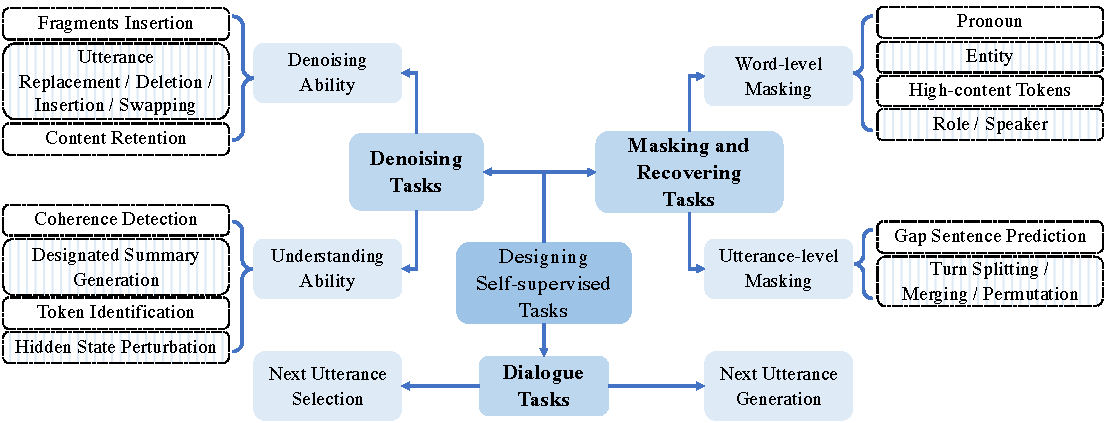
\includegraphics[scale=0.65]{fig/approach-tasks.pdf}
	\caption{A summary of self-supervised tasks.}
	\label{fig:app-task}
\end{figure}

The self-supervised tasks are summarized in Fig.~\ref{fig:app-task}. Most of them are adopted in two ways:
\begin{itemize}
	\item \textbf{Cooperating with the vanilla generation task under 
different training paradigms.}	
{Multi-task learning refers that the losses from self-supervised tasks are weighed summed with the vanilla generation for updating}~\cite{zhao2021give,fuzw20}, or updated sequentially in a batch~\cite{liu2021topic}. 
Pre-training with auxiliary tasks and then fine-tuning on dialogue summarization is also widely accepted~\cite{khalifa2021bag,qi2021improving}. 
The former is usually selected when the auxiliary training tasks are close to the summarization target. 
The latter one is chosen for learning more general representations, and is more flexible to use additional data in \secref{sec:useadddata}. 
	\item \textbf{Training an isolated model for different purposes.} 
The model is used as the summarization model directly~\cite{zou2021unsupervised, feigenblat-etal-2021-tweetsumm-dialog}, or as a trained labeler providing information for dialogue summarization~\cite{feigenblat-etal-2021-tweetsumm-dialog} with less artificial facts compared with \citet{feng2021language}. 
	
	

\end{itemize}


The advantages and disadvantages of designing self-supervised tasks are as follows:
\begin{itemize}
	\item[\Checkmark] Most self-supervised tasks take advantage of 
self-supervision to train the model. They don't need to go through
the expensive and time-consuming annotation process for collecting 
high-quality labels, and avoid the domain transfer problems 
of transferring labelers trained on the labeled domain to the target 
summarization domain.
	\item[\Checkmark] Useful representations are learned with these tasks by the summarization model directly or as an initial state for the summarization model, avoiding the error propagation caused by wrong labels. Although labeling tools such as POS tagger and TextRank are adopted, these predicted labels are not used as the training target or explicitly injected into the summarization model. They are just incorporated to find more effective self-supervisions.
	\item[\Checkmark] It's a good way to make full use of dialogue-summary 
pairs without additional labels, or even utilize pure dialogues without 
summaries.
	\item[\XSolidBrush] Although designing 
self-supervised tasks reduces the data pre-processing complexity, 
it increases the training time and computing costs with additional training targets 
on corresponding variations of the data.
	\item[\XSolidBrush] Different self-supervised tasks are not always 
compatible and controllable. It is challenging to design suitable tasks and 
find the best combination of tasks in different scenarios.
\end{itemize}



\section{Using Additional Data}\label{sec:useadddata}

Since dialogue summarization data is limited, researchers 
adopt data augmentation or borrow datasets from other tasks. 
We divide the data into two categories: 
Narrative Text and Dialogues.

\subsection{Narrative Text}

A number of {narrative text corpora} are utilized to do language modeling and learn commonsense knowledge which is shared across tasks.
Since most of today's summarization models are based on pre-trained encoder-decoder models, such as BART~\cite{lewis2020bart}, PEGASUS~\cite{zhang2020pegasus}, and T5~\cite{raffel2020exploring},  \textbf{common crawled text corpora} can be regarded as the backbone corpora of dialogue summarization. It generally includes Wikipedia, BookCorpus~\cite{zhu2015aligning} and 
C4~\cite{raffel2020exploring}. 
Pre-trained large language models on top of these corpora, such as GPT-3~\cite{brown2020language}, can be directly used for dialogue summarization with prefix-tuning approaches~\cite{prodan2021prompt}.
\citet{li2021learn} transformed such data by dividing the sequence 
into two spans, selecting span pairs with higher overlaps by Rouge scores for training their model with better copying behaviors.
The corresponding overlapped text generation task boosts their proposed model with the correlation copy mechanism on both document and dialogue summarization tasks.

Document summarization is the most similar task to dialogue summarization. As a result, \textbf{document summarization data} is a natural choice for learning the summarization ability.
\citet{zhang2021exploratory} show that BART pre-trained with 
CNN/DM~\cite{hermann2015teaching}
enhances the dialogue summarization in the meeting and drama scenarios.
CNN/DM, Gigaword~\cite{rush2015neural}, and 
NewsRoom~\cite{grusky2018newsroom} were all adopted to train a model from scratch by~\citet{zou2021low}.
For taking advantage of models trained document summarization data to do zero-shot on dialogues, \citet{ganesh2019restructuring} narrowed down the format gap between documents and dialogues by restructuring dialogue with complicated heuristic rules, such as discourse labels mentioned in \secref{sec:graphs}
Differently, \citet{zhu2020end} shuffled sentences from multiple 
documents to get a simulated dialogue for pre-training, including 
CNN/DM, XSum~\cite{narayan2018don} and NYT~\cite{evan2008nyt}.
Similarly, \citet{park2022leveraging} simulated dialogues with three transformation functions: arranging text into dialogue format by adding ``Speaker 1:'', shuffling sentence order and omitting the most extractive sentences for enhancing the abstractiveness of constructed samples.


\textbf{Commonsense knowledge data} are also welcomed as a
basis for language understanding.
\citet{khalifa2021bag} considered three reasoning tasks, including ROC stories 
dataset~\cite{mostafazadeh2016corpus} for short story ending prediction, 
CommonGen~\cite{lin2020commongen} for generative commonsense reasoning, 
and ConceptNet for commonsense knowledge base construction. 
These three tasks, together with dialogue summarization, are jointly trained and show a performance boost.
Besides, MSCOCO~\cite{lin2014microsoft} as a \textbf{short text corpus} is used in~\citet{zou2021low} for training the decoder with narrative text generation ability.


\subsection{Dialogue}

For collecting or constructing more \textbf{dialogue summarization data} 
without the need for human annotations, data augmentation approaches are 
proposed. \citet{liu2021controllable} and \citet{khalifa2021bag} augmented 
by replacing person names in both the dialogue and the reference summary 
at the same time. These augmented data are definitely well-paired and 
mixed with the original training data. 
\citet{jia-etal-2022-post} simply paired the whole dialogue with each summary sentence and further trained the model with a prefix-guided generation task before fine-tuning, where the first several tokens of the target sentence are provided for guiding the model on generation and learning to rephrase from dialogue to narrative text to some extent.
\citet{asi2022end} showed that it is possible to take advantage of giant language models such as GPT-3~\cite{brown2020language} to collect pseudo summaries by inputting dialogues with pre-defined question hints.
\citet{liu2022data} collected augmented training pairs with a small seed dataset by following steps: aligning summary spans with utterances, replacing utterances by reconstruction of the masked dialogue,
and filling up the masked summary given the augmented dialogue. 
\citet{fang2022spoken} augmented and refined the original training pairs with an utterance rewriter~\cite{liu2020incomplete} and a coreference resolution model~\cite{joshi2020spanbert}.
Besides, using relatively large-scaled crawled dialogue summarization data as 
a pre-training dataset, such as MediaSum~\cite{zhu2021mediasum}, 
for other low-resource dialogue summarization scenarios was considered by \citet{zhu2021mediasum}. 
For crawled data without summaries, \citet{yang2022tanet} constructed pseudo summaries by selecting leading comments from the long forum threads on the Reddit.




\textbf{Dialogue data} without paired summary are also valuable.
\citet{feng2020dialogue} took questions as outputs and a number of utterances after each question as inputs, regarding question generation as the pre-training objective to help identify important contents in downstream summarization. 
\citet{khalifa2021bag} adopted word-level masks on PersonaChat~\cite{zhang2018personalizing} and Reddit comments 
for fine-tuning. 
\citet{qi2021improving} pre-trained with dialogues from MediaSum and TV4Dialogue besides document summarization datasets used in \citet{zhu2020end}. They also stitch dialogues randomly to simulate topic transitions. 
\citet{zhong2021dialoglm} proposed a generative pre-training framework for long dialogue understanding and comprehension. DialogLM in this work is specially pretrained on dialogues from MediaSum dataset and OpenSubtitles Corpus~\cite{lison2016opensubtitles2016}. It corrupts a window of dialogue utterances with dialogue-inspired noises, similar to the noising operations mentioned in \secref{sec:designselftasks}. 
The original window-sized utterances are the recovering target based on the remaining dialogue. Such a window-based recovering task is suggested to be more suitable for dialogues considering its scattered information and highly content-dependent utterances. 
Besides, \citet{amanda-etal-2022-shift} took advantage of a self-annotated corpus based on SAMSum~\cite{gliwa2019samsum} which converts each utterance individually to a third-person rephrasing.
They showed benefits on the same dataset under the zero-shot setting by pre-training with this perspective shift corpus.


Furthermore, \citet{zou2021low} broke the training for dialogue summarization 
model into three parts, namely encoder, context encoder and decoder, 
to train the dialogue modeling, summary language modeling and 
abstractive summarization respectively. 
Dialogue corpus, short text corpus, and summarization corpus were all 
used in this work, helping to bridge the gap between out-of-domain 
pre-training and in-domain fine-tuning, especially for low-resource settings.
	
\subsection{Summary and Opinions}

\begin{figure}
	\centering
	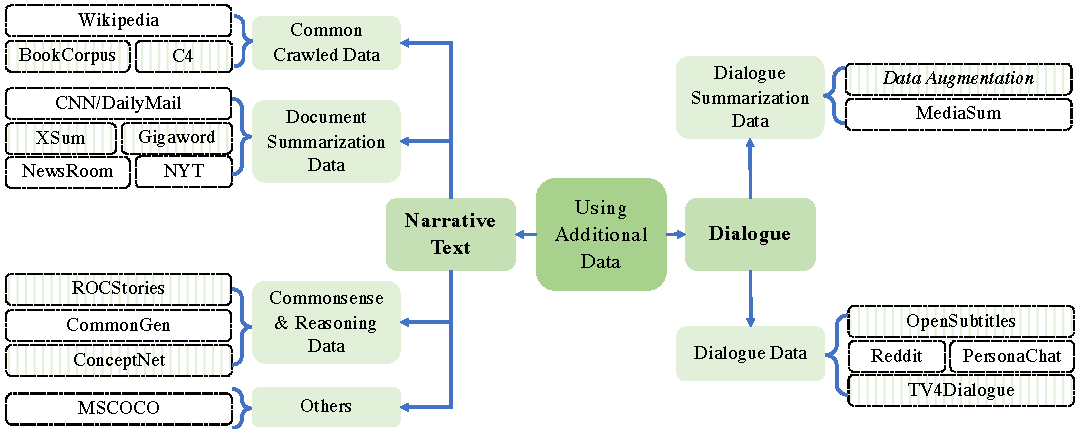
\includegraphics[scale=0.65]{fig/approach-data.pdf}
	\caption{A summary of additional data.}
	\label{fig:app-data}
\end{figure}

Additional data in previous work are in Fig.~\ref{fig:app-data}. These data are always used in the following ways:
\begin{itemize}
	\item \textbf{Pre-training with corresponding training objectives}. 
Common crawled text data, document summarization data and dialogue data are 
mostly used in this way~\cite{zou2021low}, where the language styles or data 
formats are quite different from dialogue-summary pairs. It hopes to 
provide a better initialization state of the model for dialogue summarization. 
On the other hand, it is also a good way for coarse-to-fine-grained training, 
where pre-training is done with the noisy data by data augmentation or from other 
domains and fine-tuning with the oracle dialogue summarization training data~\cite{feng2020dialogue,zhu2021mediasum}.


\item \textbf{Mixing with dialogue summarization training data} and 
training for dialogue summarization directly. 
Data here are usually more similar to dialogue-summary pairs obtained by data 
augmentation~\cite{liu2021controllable,khalifa2021bag} or with intensive 
commonsense~\cite{khalifa2021bag,liu2022data}. 
\end{itemize}

The advantages and disadvantages of using additional data are as follows:
\begin{itemize}
	\item[\Checkmark] The language understanding ability among different 
corpora is the same intrinsically. As a result, additional data helps 
dialogue summarization, especially in low-resource settings, 
which further alleviates the burden of summary annotation by humans.
	\item[\Checkmark] The intensive knowledge in specially designed 
corpora helps strengthen the dialogue summarization model. 
	\item[\Checkmark] The additional unlabeled data can be trained 
with self-supervised tasks mentioned in \secref{sec:designselftasks} for 
better performance.
	\item[\XSolidBrush] Training with additional data makes significant improvements while requiring 
more time and computational resources, reflecting the data inefficiency of current models.
	\item[\XSolidBrush] Training with more data is not always effective~\cite{zhang2021exploratory,nair2021data}, especially when the divergence between 
the additional corpus and original dialogue summarization corpus is huge.  Elaborate data augmentation approaches avoid this problem when training data is not too scarce.
\end{itemize}
	

\section{Evaluations}
\label{sec:evaluation}

In this section, we present a comprehensive description of existing dialogue summarization datasets 
under different scenarios and introduce several widely-accepted evaluation 
metrics for this task.
%The benchmark and some of these dataset have been concluded in \cite{feng2021survey}. So, we mainly organize features above that have been proven to be helpful for different scenarios.

\subsection{Datasets}
\label{sec:dataset}

A great number of dialogue summarization datasets have been proposed from different resources. We categorize them according to the scenarios in Section \ref{sec:scenarios}. %as shown in Figure~\ref{fig:scenario}.


\subsubsection{Open-domain Dialogue Summarization}

Open-domain dialogue summarization datasets under daily chat, drama conversation and debate\&comment are as follows and summarized in Table~\ref{tab:open}.

\textit{Daily Chat Datasets}: \textbf{SAMSum}~\cite{gliwa2019samsum} and \textbf{DialogSum}~\cite{chen2021dialsumm} are two large-scale real-life labeled datasets. Each dialogue in SAMSum is written by one person to simulate a real-life 
messenger conversations and the single reference summary is annotated by 
language experts. DialogSum, on the other hand, contains dialogues from 
the existing dialogue dataset, including DailyDialog~\cite{li2017dailydialog}, 
DREAM~\cite{sun2019dream} and MuTual~\cite{cui2020mutual}, and other English-speaking practice websites. These spoken dialogues have a more formal style than those in SAMSum, and each is accompanied by three reference summaries in the test set.  %\citet{chen2021dialsumm} claims that DialSumm is a more challenging dataset with a lower compression ratio and more diverse topics than SAMSum. 
Besides, AIHub Dialogue Summarization Dataset (\textbf{HubDial})~\footnote{https://aihub.or.kr/} also contains dialogues covering a range of daily topics.

 
%Dramatic dialogues represent the dialogues on TV which are likely to have drama scripts behind them.
\textit{Drama Conversation Datasets}: \textbf{CRD3}~\cite{rameshkumar2020storytelling} is collected from a live-stream role-playing game called Dungeons and Dragons, which is more amenable to extractive approaches with low abstractiveness.
%The dataset consists of 159-episode dialogue transcripts and summaries with extremely long texts, and they further segment paired texts into dialogue-summary chunks with reasonable lengths for training with neural networks. 
%CRD3 is more amenable to extractive approaches with low abstractiveness.
 \textbf{MediaSum}~\cite{zhu2021mediasum} includes interview transcripts from 
NPR and CNN and their reviews or topic descriptions are regarded as the 
corresponding summaries. The large size of this automatically crawled 
dataset makes it particularly suitable for pre-training. %for zero-shot or few-shot applications.
Other two datasets are collected from a variety of movies and TV series, 
including \textbf{SubTitles}~\cite{malykh2020sumtitles} and 
\textbf{SummScreen}~\cite{chen2021summscreen}. Dialogues are corresponding 
transcripts, and summaries are aligned synopses or recaps 
written by humans.
%According to dataset styles and dialogue-summary aligning approaches, \textbf{SubTitles}~\cite{malykh2020sumtitles} consists of Subtitiles, Scripts and Gold, and \textbf{SummScreen}~\cite{chen2021summscreen} consists of TMS and FD. 
%The alignment in Scripts are done automatically with multiple similarity functions, while Gold are done by human annotators.
%Summaries form Subtitles are high-level plot summaries describing a movie or a series episode in no more than ** words compared with Scripts and Gold.
%TMS focus more on dialogues with more details in the corresponding summaries, while FD have more descriptions about environments or character actions with shorter summaries.
 
%Dialogues rich in discussions and comments are also a representative application scenario. For example, people may discuss about politics or world affairs online after they go through the corresponding news.
%Summarizing such dialogues helps people know better about the world.
 \textit{Debate\&Comment Datasets}: \textbf{ADSC}~\cite{misra2015using} 
is a test-only dataset extracted from the Internet Argument 
Corpus~\cite{walker2012your}. It contains 45 two-party dialogues about gay 
marriages, each  associated with 5 reference summaries. 
\textbf{FORUM}~\cite{tarnpradab2017toward} contains human-annotated forum threads collected from tripadvisor.com and ubuntuforums.org.
Three out of four sub-datasets in \textbf{ConvoSumm}~\cite{fabbri2021convosumm} 
are similar discussions, including news article comments (\textbf{NYT}), 
discussion forums and debate (\textbf{Reddit}) and community question answers 
(\textbf{Stack}) from different sources. Each sample has a human-written reference.
\textbf{CQASUMM}~\cite{chowdhury2019cqasumm} is another community question 
answering dataset but without back and forward discussions among speakers. The summary here aims to summarize multiple answers, which is closer to a multi-document summarization setting.
% which is more similar to \KZ{rephrase: a multi-document summarization setting among answers without discussions between multiple interlocutors.}%The labeled summaries are relative small with 250 development and 250 test examples respectively.

\begin{table}[th]
	\centering
	\small
		\begin{tabular}{|l|c|c|c|c|c|p{4cm}|c|}
			%|l|c|c|c|c|c|c|
			\hline
			\textbf{\makecell[c]{Name}} & \textbf{\makecell{$\#$Samples \\ train/val/test}} & \textbf{$\#$Spk} & \textbf{Lang.} & \textbf{DW} & \textbf{SW} & \textbf{\makecell[c]{Download Link}} & \textbf{AVL} \\
			\hline
			\multicolumn{6}{|l|}{\bf \em{Daily Chat}} \\
			\hline
			%\tabincell{c}{SAMSum\cite{gliwa2019samsum}} & 14,732/818/819 & $\geq$2 & Eng. & \tabincell{l}{https://www.tensorflow.org/\\datasets/catalog/samsum}& Y \\
			%\hline
			SAMSum\cite{gliwa2019samsum} & 14.7k/0.8k/0.8k%14,732/818/819 
			& $\geq$2 & English & 94 & 25 & \tabincell{l}{https://huggingface.co/datasets\\/samsum}& Y \\
			\hline
			DialogSum\cite{chen2021dialsumm} & 12.5k/0.5k/0.5k%12,460/500/500 
			& 2& English & 131 & 22 &\tabincell{l}{https://github.com/cylnlp/\\DialogSum} & Y\\
			
			\hline
			HubDial & 350k & $\geq$2 & Korean & - & - &\tabincell{l}{https://aihub.or.kr/}  & C \\
			
			\hline
			%GupShup\cite{mehnaz2021gupshup} & 5.8k/0.5k/0.5k %5,831/500/500
			%& $\geq$2 &  \tabincell{l}{Hindi-\\English} & ** & ** & \tabincell{l}{https://huggingface.co/\\midas/gupshup\_h2e\_mbart} &Y \\
			%\hline
			\multicolumn{6}{|l|}{\bf \em{Drama Conversation}} \\
			\hline
			CRD3\cite{rameshkumar2020storytelling} &	26.2k/3.5k/4.5k %26,232/3,470/4,541 
			& $\geq$2 & English & 31,803 & 2,062 & \tabincell{l}{https://github.com/\\RevanthRameshkumar/CRD3}& Y \\
			\hline
			MediaSum\cite{zhu2021mediasum} &
			463.6k/10k/10k %463,6000/10,000/10,000
			& $\geq$2 & English & 1,554 & 14 & \tabincell{l}{https://github.com/\\zcgzcgzcg1/MediaSum/}& Y \\
			\hline
			\makecell[l]{SumTitles\cite{malykh2020sumtitles}\\(Subtitiles/Scripts/Gold)} & \makecell[c]{132k\\21k\\290}%153k 
			& $\geq$2 & English & \makecell[c]{6,406\\423\\395} & \makecell[c]{85\\55\\51} & \tabincell{l}{https://github.com/huawei-\\noah/noah-research/tree/\\master/SumTitles}& Y \\
			\hline
			\makecell[l]{SummScreen\cite{chen2021summscreen}\\(FD/TMS)} &\makecell[c]{3,673/338/337\\18,915/1,795/1,793} %22.6k/2.1k/2.1k %22,588/2,133/2,130
			& $\geq$2 & English & \makecell[c]{7,605\\6,421} & \makecell[c]{114\\381} & \tabincell{l}{https://github.com/mingdachen\\/SummScreen}& Y \\
			\hline
			\multicolumn{6}{|l|}{\bf \em{Debate \& Comment}} \\
			\hline
			ADSC\cite{misra2015using} & 45 & 2 & English & 672 & 151 &\tabincell{l}{https://nlds.soe.ucsc.edu/\\summarycorpus}& Y \\
			\hline
			CQASUMM\cite{chowdhury2019cqasumm} & 100k
			& $\geq$2 & English& 782 & 100 &\tabincell{l}{https://bitbucket.org/tanya1410\\9/cqasumm/src/master/} & Y\\
			
			\hline
			FORUM~\cite{tarnpradab2017toward} & 689 & $\geq$2 & English & 825 & 191 &  \tabincell{l}{http://tinyurl.com/jcqgcu8} & Y \\
			
			\hline
			\makecell[l]{ConvoSumm\cite{fabbri2021convosumm}\\(NYT/Reddit/Stack)} &  \makecell[c]{-/0.25k/0.25k\\-/0.25k/0.25k\\-/0.25k/0.25k}
			& $\geq$2 &  \tabincell{l}{English}& \makecell[c]{1,624\\641\\1,207} & \makecell[c]{79\\65\\73} & \tabincell{l}{https://github.com/\\Yale-LILY/ConvoSumm} &Y \\
			
			\hline
			
		\end{tabular}
		\caption{Open-domain dialogue summarization datasets. ``Lang.''  and ``Spk'' stands for ``Language'' and ``Speakers''. ``DW'' and ``SW'' represents the average number of words in the dialogues and summaries respectively. ``AVL'' refers to the public availability of the
dataset ($Y$ is available, $N$ is not available, and $C$ is conditional). HubDial is only available for Koreans.}%\JQ{the average source content length (word and utterance) and summary length in Table 1 and Table 2}}
%\KZ{Change D to C (conditional)?}}	
		\label{tab:open}		
\end{table}


\subsubsection{Task-oriented Dialogue Summarization}

Datasets here are rooted in specific domains, including
customer service, law, medical care and official issue. We list them in Table~\ref{tab:task}. 

%With the rapid development of Internet services, online customer service becomes important increasingly. 
%In the e-commerce scenario,
\textit{Customer Service Datasets}: Zou et al.\shortcite{zou2021topic,zou2021unsupervised} propose two similar datasets with summaries from the agent perspective.
\citet{lin2021csds} provides a more fine-grained dataset \textbf{CSDS} containing a user summary, an agent summary, and an overall summary based on JDDC dataset~\cite{chen2020jddc}. %\citet{zou2021unsupervised} also mentioned a similar dataset.
Summaries from \textbf{Didi dataset}~\cite{liu2019automatic} are also written from agents' points of view, in which dialogues are about transportation issues instead of pre-sale and after-sale topics in the former one.
More complicated multi-domain scenarios are covered in \textbf{TWEETSUMM}~\cite{feigenblat-etal-2021-tweetsumm-dialog}, \textbf{MultiWOZ*}~\cite{yuan2019scaffolds} and \textbf{TODSum}~\cite{zhao2021todsum}. Dialogues from TWEETSUMM spread over a wide range of domains, including gaming, airlines, retail, and so on. 
MultiWOZ* and TODSum transform and annotate summaries based on the original MultiWOZ dataset~\cite{eric2019multiwoz}.
There are also two earlier datasets called \textbf{DECODA} and \textbf{LUNA}~\cite{favre2015call} containing call centre conversations with synopses summarizing the problem of the caller and how it is solved.  
%\KZ{What does this mean: contains domain transitions and inherent domain ontology within a dialogue}.
%Dialogues in this dataset are collected based on (domain, intent, slot, value) tuples according to a structured ontology based on domain knowledge.




\begin{table}[t]
	\centering
	\small		
		\begin{tabular}{|l|c|c|c|c|c|p{3.7cm}|c|}
			\hline
			\textbf{\makecell[c]{Name}} &\textbf{ \makecell{$\#$Samples \\ train/val/test}}& \textbf{$\#$Spk} & \textbf{Lang.} & \textbf{DW} & \textbf{SW} & \textbf{\makecell[c]{Download Link}} & \textbf{AVL} \\
			\hline
			\multicolumn{6}{|l|}{\bf \em{Customer Service}} \\
			
			\hline
			\citet{zou2021topic} & 17.0k/0.9k/0.9k%18.86k 90%/5%/5% 
			& 2 & Chinese & 1,334 & 55 &\tabincell{l}{https://github.com/RowitZou\\/topic-dialog-summ}& Y \\
			
			\hline
			CSDS\cite{lin2021csds} & 9.1k/0.8k/0.8k%9,101 / 800 / 800
			& 2& Chinese & 401 & 83 &\tabincell{l}{https://github.com/xiaolin\\Andy/CSDS} & Y\\
			
			\hline
			{\citet{zou2021unsupervised}} & -/0.5k/0.5k%1.09M chat logs
			& 2 &  \tabincell{l}{Chinese}& 95 & 37 & \tabincell{l}{https://github.com/RowitZou\\/RankAE} &Y \\
			
			\hline
			{Didi\cite{liu2019automatic}} &296.3k/2.9k/29.6k %26,232/3,470/4,541 
			& 2 & Chinese & - & - &	\tabincell{l}{-}& N \\
			
			\hline
			{TWEETSUMM\cite{feigenblat-etal-2021-tweetsumm-dialog}} & 0.9k/0.1k/0.1k %1.1k 80%/10%/10%
			& 2 & English & 245 & 36 & \tabincell{l}{https://github.com/guyfe\\/Tweetsumm}& Y \\
			
			
			\hline
			MultiWOZ*\cite{yuan2019scaffolds} & 8.3k/1k/1k & 2 & English & 181 & 92 & \tabincell{l}{https://github.com/voidforall\\/DialSummar}& Y\\
			
			\hline
			{TODSum\cite{zhao2021todsum}} & 9.9k & 2 & English & 187 & 45 &\tabincell{l}{-}& N \\
			
			\hline
			DECODA\cite{favre2015call} & -/50/100 & 2 & \makecell[c]{French/\\English}
			& \makecell[c]{42,130\\41,639} & \makecell[c]{23\\27} & \tabincell{l}{https://pageperso.lis-lab.fr/\~benoit\\.favre/cccs/} & C\\
			
			\hline
			LUNA\cite{favre2015call} & -/-/100 & 2 & \makecell[c]{Italian/\\English}
			& \makecell[c]{34,913\\32,502} & \makecell[c]{17\\15}  &\tabincell{l}{https://pageperso.lis-lab.fr/\~benoit\\.favre/cccs/}  & C\\
			
			\hline
			\multicolumn{6}{|l|}{\bf \em{Law}} \\
			
			\hline
			{Justice\cite{fuzw20}} & 30k%14,732/818/819 
			& 2 & Chinese & 605 & 160 & \tabincell{l}{-}& N \\
			
			\hline
			{PLD\cite{duan2019legal}} & 5.5k& $\geq$2 & English  & - & - &\tabincell{l}{https://github.com/zhouxinhit\\/Legal\_Dialogue \_Summarization} & C \\
			
			\hline
			{LCSPIRT-DM\cite{xi2020global}} &  30.8/3.8k/3.8k%38.5k 80%/10%/10%
			& 2 &  Chinese& 684 & 75 & \tabincell{l}{http://eie.usts.edu.cn/prj/\\NLPoSUST/LcsPIRT.htm} & C \\
		
			\hline
			\multicolumn{6}{|l|}{\bf \em{Medical Care}} \\
		
			\hline
			{\citet{joshi2020dr}} & 1.4k/0.16k/0.17k%1365 /158/167 
			& 2 & English & - & - &\tabincell{l}{-}& N \\
			
			\hline
			{\citet{song2020summarizing}} & 36k/-/9k %35987/8996
			& 2& Chinese  & 312 & 23/113 &\tabincell{l}{https://github.com/cuhksz-nlp\\/HET-MC} & Y\\
			
			\hline
			{\citet{liu2019topic}} & 100k/1k/0.49k
			& 2 &  \tabincell{l}{English}& - & - & \tabincell{l}{-} &N \\
			
			\hline
			{\citet{zhang2021leveraging}} & 0.9k/0.2k/0.2k %939(15043), 201(3095), and 202(3450),
			& 2 & English & - & - & \tabincell{l}{-}& N \\
			
			\hline
			\multicolumn{6}{|l|}{\bf \em{Official Issue (Meeting \& Emails)}} \\
			
			\hline
			{AMI\cite{carletta2005ami}} &137 %142 
			& $>$2 & English & 4,757 & 322 & \tabincell{l}{https://groups.inf.ed.ac.uk/ami}& Y \\
			
			\hline
			{ICSI\cite{janin2003icsi}} & 59 %75 
			& $>$2 & English & 10,189 & 534 &\tabincell{l}{https://groups.inf.ed.ac.uk/ami\\/icsi}& Y \\
			
			\hline
			{QMSum\cite{zhong2021qmsum}} & 1.3k/2.7k/2.7k% 1,257 / 272 / 279 
			& $>$2 & English & 9070 & 70 &\tabincell{l}{https://github.com/Yale-LILY\\/QMSum}& Y \\
			
				\hline
			{Kyutech\cite{yamamura2016kyutech,nakayama2021corpus}} &  9 
			& $>$2 & Japanese & - & - &\tabincell{l}{http://www.pluto.ai.kyutech.\\ac.jp/~shimada/resources.html}& Y \\
			
			\hline
			{BC3\cite{ulrich2008publicly}} & 30%1800/249/500
			& $>$2 & English & 550 & 134 &\tabincell{l}{https://www.cs.ubc.ca/cs-\\research/lci/research-groups\\/natural-language-processing\\/bc3.html} & Y \\
			
			\hline
			{\citet{loza2014email}} & 107%1800/249/500
			& $>$2 & English & - & - &\tabincell{l}{-} & N\\
			
			\hline
			{EmailSum\cite{zhang2021emailsum}} & 1.8k/0.25k/0.5k%1800/249/500
			& $\geq$2 & English& 233 & 27/69 &\tabincell{l}{https://github.com/ZhangShiyue\\/EmailSum} & C \\
			
			\hline
			\makecell[l]{ConvoSumm\cite{fabbri2021convosumm}\\(Email)} &  -/0.25k/0.25k%
			& $\geq$2 &  \tabincell{l}{English} &917 & 74 & \tabincell{l}{https://github.com/Yale-LILY\\/ConvoSumm} &Y \\
			
			\hline
		
		\end{tabular}	
		\caption{Task-oriented dialogue summarization datasets. The original text data is not accessible for PLD due to privacy issues. DECODA, LUNA and LCSPIRT-DM can only be obtained through an application. EmailSum is not free.}
		\label{tab:task}
	%\caption{Dialogue Summarization Datasets}	
\end{table}


%Courts and police are meaningful scenarios for releasing the rising workload.
\textit{Law Datasets}: \textbf{Justice}~\cite{fuzw20} includes 
debates between a plaintiff and a defendant on some controversies 
which take place in the courtroom. The final factual statement by the 
judge is regarded as the summary.
A similar scenario is included in \textbf{PLD}~\cite{duan2019legal}, which is more 
difficult to summarize due to the unknown number of participants. There is also another version 
of PLD by~\citet{gan2021inspectional} with fewer labeled cases than the 
original PLD.
\citet{xi2020global} proposed a long text summarization dataset \textbf{LCSPIRT-DM} based 
on police inquiry records full of questions and answers.


\textit{Medical Care Datasets}:
%Medical care are heath consultation dialogues between doctors and patients. 
Both \citet{joshi2020dr} and \citet{song2020summarizing} proposed medical summarization corpora by crawling data from online health platforms and annotating coherent summaries by doctors. \citet{song2020summarizing} also proposed one-sentence summaries of medical problems uttered by patients, whereas \citet{liu2019topic} used simulated data with summary notes in a very structured format.
 \citet{zhang2021leveraging} used unreleased dialogues with coherent summaries of the history of the present illness. %which is less structured.

%Official affairs are familiar in work. Most of them are face-to-face real-time meetings, resulting in verbose transcripts. Summarizing keynotes among the meeting can enhance the efficiency of work. 
\textit{Official Issue Datasets}: \textbf{AMI}~\cite{carletta2005ami} and \textbf{ICSI}~\cite{janin2003icsi} are meeting transcripts concerning 
computer science-related issues in working background and research background, respectively. Both datasets are rich in human labels, including extractive summary, abstractive summary, topic segmentation, and so on. They are also included in \textbf{QMSum}~\cite{zhong2021qmsum} and are further labeled for query-based meeting summarization. \textbf{Kyutech}~\cite{yamamura2016kyutech} is a similar dataset in Japanese containing multi-party conversations, where the participants pretend to be managers of a virtual shopping mall in a virtual city and do some decision-making tasks. Their later work~\cite{nakayama2021corpus} annotated more fine-grained summaries for each topic instead of the whole conversation in ~\cite{yamamura2016kyutech}.
In addition, official communications are also prevalent in e-mails. 
\citet{ulrich2008publicly} propose the first email summarization dataset \textbf{BC3} with only 30 threads and \citet{loza2014email} release 107 email threads. Both of them contain extractive as well as abstractive summaries.
EmailSum~\cite{zhang2021emailsum} has both a human-written short summary and a long summary for each e-mail thread. 
Besides, Email threads (\textbf{Email}) in ConvoSumm~\cite{fabbri2021convosumm} have only one abstractive summary for each dialogue.


\subsubsection{Summary}
We make the following observations and conclusions.
\begin{itemize}
	\item The size of dialogue summarization datasets is much smaller than document summarization datasets. Most dialogue summarization datasets have no more than $30K$ samples, while representative document summarization datasets, such as CNNDM and XSum, have more than $200K$ samples. Datasets for drama conversations are relatively larger and can be potential pre-training data for other scenarios.
%	\KZ{Try to avoid passive voice: which are potentially to be used} as pre-training data for other scenarios.
	\item The number of interlocutors in different dialogue summarization scenarios is different. Most ODS dialogues have more than $2$ speakers while 
most dialogues in TDS have only 2 speakers except in official meetings or 
e-mails.
	\item TDS dialogues tend to be more private. Thus, half of the 
TDS datasets are not publicly available, especially for Law and 
Medical Care scenarios. 
	\item Datasets with more than 2,048 dialogue words, which is the upper bound of the input length of most pre-trained language models, are suitable for research on long dialogue summarization. They contain both open-domain datasets and task-oriented datasets. 
	 %including CRD3~\cite{rameshkumar2020storytelling}, MediaSumm~\cite{zhu2021mediasum}, SumTitles~\cite{malykh2020sumtitles}, SummScreen~\cite{chen2021summscreen} and ConvoSumm~\cite{fabbri2021convosumm}, and task-oriented datasets including AMI~\cite{carletta2005ami}, ICSI~\cite{janin2003icsi}, QMSum~\cite{zhong2021qmsum} and~\citet{zou2021topic}'s customer service dataset.
	%It points out a need of a taxonomy on different techniques instead of listing approaches under different datasets, which should be more effective when facing a new scenarios with some collected data. 
\end{itemize} 
 


%\subsection{Privacy Concerns}
%Due to privacy and ethical issues of dialogues, 
%different focus on different extract or abstract, faithfulness

\subsection{Evaluation Metrics}
\label{sec:evalmetric}
In existing works, \textit{Automatic evaluation metrics} commonly used for summarization such as \textbf{Rouge}~\cite{lin2004rouge}, \textbf{MoverScore}~\cite{zhao2019moverscore}, \textbf{BERTScore}~\cite{zhang2019bertscore} and \textbf{BARTScore}~\cite{yuan2021bartscore} are also used for dialogue summarization by comparing the generations with references. However, these widely-accepted metrics' performance may deviate from human~\cite{chen2021dialsumm,hanna2021fine}, especially in the aspect of consistency. Therefore, more focussed evaluation metrics and human evaluations emphasizing \textit{information coverage} and \textit{factual consistency} are considered as follows.
%\KZ{To complement these metrics qualifying the overall matching degree to the 
%reference}, 

Instead of comparing only with the whole reference summary, most researches for TDS only consider key words/phrases
while ignoring other common words for measuring the \textbf{information coverage}.  In other words, evaluation for TDS emphasizes the coverage of key information which are generally domain-specific terms and can be easily recognized.
%moves towards accurate summaries 
For example, {medical concept coverage}~\cite{joshi2020dr,zhang2021leveraging} 
and {critical information completeness}~\cite{yuan2019scaffolds} both
extract essential phrases based on domain dictionaries by 
rules or publicly available tools. 
\citet{zhao2021give} uses slot-filling model~\cite{chen2019bert} to recognize slot values for {factual completeness}.
Then, the accuracy or F1 scores are 
calculated by comparing extracted phrases or concepts from $Y$ and $Y'$. 



%Besides these extraction-based metrics, reference-free evaluation metrics~\cite{shao2017efficient,durmus2020feqa,egan2022play,liu2022reference} are gaining more and more attention. 
%Some of them have been adopted for dialogue summarization for measuring \textbf{the factual consistency} of generations given source dialgoue.

ODS pays less attention to information coverage due to the higher subjectivity on salient information selection. Instead, measuring the \textbf{factual consistency} of generations gains increasing attention. Unlike the above metrics which compare generations with the reference summary, 
most evaluation metrics here compare generations with the source dialogue and can be classified into reference-free evaluation metrics~\cite{shao2017efficient,durmus2020feqa,egan2022play,liu2022reference}.
A QA-based model~\cite{wang2020asking} is borrowed by \citet{zhao2021give}.
It follows the idea that factually consistent summaries and documents generate the same answers to a question.
NLI-based methods~\cite{maynez2020faithfulness} that require the content in the summary to be fully inferred from the dialogue were adopted by~\citet{liu2022data}.
\citet{liu2021controllable} automatically evaluate {inconsistency} issues 
of person names by using noised reference summaries as negative samples and training a BERT-based binary classifier.
\citet{asi2022end} used the FactCC metric from~\citet{kryscinski2020evaluating} where the model was trained only with source documents with a series of rule-based transformations.
Information correctness of the generated summary is also important for TDS. For instance, negation correctness as a specific consistency type is considered by ~\citet{joshi2020dr} with 
publicly available tools Negex~\cite{harkema2009context} for recognizing 
negated concepts.

Meanwhile, \textit{human evaluations} are required to complement the above metrics.
Besides ranking or scoring the generated summary with an overall quality score~\cite{chen2020multi}, 
more specific aspects are usually provided to annotators. Representative ones include:
\textbf{readability/fluency}~\cite{yuan2019scaffolds,zhao2021give} requiring a summary to be grammatically correct and well structured,
\textbf{informativeness}~\cite{feng2020dialogue,lei2021finer,feigenblat-etal-2021-tweetsumm-dialog,feng2021language} measuring how well the summary includes salient information,
\textbf{conciseness/non-redundancy}~\cite{feng2021language,yuan2019scaffolds} pursuing a summary without redundancy,
and \textbf{factualness/consistency}~\cite{feng2020dialogue,zhao2021give,lei2021finer,kim2022mind} evaluating whether the summary is consistent with the source dialogue. There are also some typical fine-grained metrics evaluating errors in generated summaries mentioned in previous works~\cite{chen2020multi,chen2021dialsumm,liu2021coreference}: 
\textbf{Information missing} means that content mentioned in references are missing in generated summaries, while \textbf{information redundancy} is the opposite.
\textbf{Reference error} refers to wrong associations between a speaker and an action or a location.
\textbf{Reasoning error} is that the model incorrectly reasons the conclusion among multiple dialogue turns.
Moreover, \citet{chen2020multi} mentioned \textbf{improper gendered pronouns} referring to improper gendered pronouns. \citet{tang2021confit} also proposed \textbf{circumstantial error}, \textbf{negation error}, \textbf{object error}, \textbf{tense error} and \textbf{modality error} for more detailed scenarios. All of their error types can also be grouped into two classes, where the information missing and redundancy are for the coverage of key information, and the rest are for factual consistency.


A summary of evaluation metrics adopted in existing dialogue summarization works is in Table~\ref{tab:eval-metrics}.

\begin{table}[h]
	\centering
	\small
	\begin{tabular}{|l|l|p{6.8cm}|}
		\hline
		\textbf{Types} & \textbf{Description} & \textbf{Metrics} \\
		\hline
		\multirow{3}{*}{Automatic Evaluation} & Commonly-used & Rouge, MoverScore, BERTScore, BARTScore, ... \\
		\cline{2-3}
		 & Information Coverage & medical concept coverage, critical information completeness, factual completeness, ...\\
		 \cline{2-3}
		 & Factual Consistency & QA-based metrics, NLI-based metrics, binary classifiers with synthetic data, negation correctness, ...\\
		 \hline
		\multirow{3}{*}{Human Evaluation} & Evaluation Aspects& readability / fluency, informativeness, conciseness / non-redundancy, factualness / consistency\\
		\cline{2-3}
		& Error Types & {information missing, information redundancy, reference error, reasoning error, improper gendered pronouns, circumstantial error, negation error, object error, tense error, modality error} \\ 
		\hline
		
	\end{tabular}
	\caption{A summary of evaluation metrics.}
	\label{tab:eval-metrics}
\end{table}

%including readability/fluency~\cite{yuan2019scaffolds,zhao2021give}, completeness~\cite{lei2021finer}, informativeness~\cite{feng2020dialogue,lei2021finer,feigenblat-etal-2021-tweetsumm-dialog,feng2021language}, conciseness/non-redundancy~\cite{yuan2019scaffolds}, consistency/factualness~\cite{feng2020dialogue,zhao2021give,lei2021finer} and coherence.
%Information missing, information redundant, reference error, reasoning error, 
%improper gender pronouns and tense consistency are typical fine-grained metrics evaluating 
%errors in generated summaries.

%Some specially designed metrics are introduced for specific purpose, such as medical concept coverage~\cite{joshi2020dr,zhang2021leveraging} and negation correctness~\citet{joshi2020dr} which are important factors contributing to accurate medical summaries. These evaluating targets are extracted either utilizing domain dictionaries with rules or publicly available tools, such as quickUMLS~\footnote{\url{https://www.nlm.nih.gov/research/ umls/index.html}} for medical concepts and Negex~\cite{harkema2009context} for recognizing negated concepts. 
%\citet{zhao2021give} propose factual consistency and factual completeness based on pretrained QA-based model~\cite{wang2020asking} and slot-filling model~\cite{chen2019bert}.
%\citet{liu2021controllable} trains a BERT-based binary classifier for detecting inconsistency issues of person names between dialogues and the summaries. 

%\citet{yuan2019scaffolds} proposed Critical Information Completeness for computing the matched predefined essential entities or slots in $Y$ and $Y'$, ignoring other common words or phrases.

%\cut{%%%%%
%\begin{sidewaystable}
\begin{table}
\centering
\subtable[Open-domain Dialogue Summarization]{	
\begin{tabular}{|ccccp{3cm}<{\centering}p{2cm}<{\centering}c|}
	%|l|c|c|c|c|c|c|
	\hline
	Name & \makecell{$\#$Samples \\ train/val/test} & $\#$Speakers & Lang. & Desc. & Down. & AVL \\
	\hline
	\multicolumn{7}{|l|}{\bf \em{Dialy Chats}} \\
	\tabincell{c}{SAMSum\cite{gliwa2019samsum}} & 14,732/818/819 & $\geq$2 & Eng. & \tabincell{l}{Dialogues and gold \\ summaries in dataset \\ are human-annotated.}& \tabincell{l}{https://www.\\tensorflow.org/\\datasets/catalog/\\samsum}& Y \\
	\makecell{DialSumm\cite{chen2021dialsumm}} & & & & & & \\
	\makecell{GupShup\cite{mehnaz2021gupshup}} & & & & & & \\
	
	\hline
			
\end{tabular}	
\label{tab:open}		
}
\qquad
\subtable[Task-oriented Dialogue Summarization]{        		
\begin{tabular}{|l|c|c|c|c|c|c|}
\hline
Name & $\#$Samples & $\#$Speakers & Lang. & Desc. & Down. & available \\
\hline
\end{tabular}	
\label{tab:task}
}
\caption{Dialogue Summarization Datasets}	
\end{table}
%\end{sidewaystable}
}%%%%%


\begin{sidewaystable}[thp]
	    \centering
	    \rule{0\textheight}{0.7\textheight}
		\begin{tabular}{|c|c|c|c|l|l|c|}

			\hline
			Name & \makecell{$\#$Samples \\ train/val/test} & $\#$Speakers & Language & Description & Download & AVL \\
			\hline
			\multicolumn{7}{|l|}{\bf \em{Dialy Chats}} \\
			\hline
			\tabincell{c}{SAMSum\cite{gliwa2019samsum}} & 14.7k/0.8k/0.8k%14,732/818/819 
			& $\geq$2 & English & \tabincell{l}{Dialogues and gold summaries in dataset  \\are human-annotated.}&
			 \tabincell{l}{https://huggingface.co/\\datasets/samsum
			 	%https://www.tensorflow.org/\\datasets/catalog/samsum
		 	}& Y \\
			 \hline
			\makecell{DialSumm\cite{chen2021dialsumm}} & 12.5k/0.5k/0.5k%12,460/500/500 
			& 2& English &\tabincell{l}{Dialogue data are collected from public \\dialogue corpora and each dialogue has 3 \\manually annotated reference summaries.} &\tabincell{l}{https://github.com/cylnlp/\\DialogSum} & Y\\
			\hline
			\makecell{GupShup\cite{mehnaz2021gupshup}} & 5.8k/0.5k/0.5k %5,831/500/500
			& $\geq$2 &  \tabincell{l}{Hindi-\\English}& \tabincell{l}{The dialogues and summaries are \\sampled from SAMSum and manually \\translated from English to Hindi-English.}& \tabincell{l}{https://huggingface.co/\\midas/gupshup\_h2e\_mbart} &Y \\
			\hline
			\multicolumn{7}{|l|}{\bf \em{Dramatic Dialogues}} \\
			\hline
			\tabincell{c}{CRD3\cite{rameshkumar2020storytelling}} &
			26.2k/3.5k/4.5k %26,232/3,470/4,541 
			& $>$2 & English & \tabincell{l}{Dialogues and  summaries are collected \\ from {\em Critical Role} episode and Fandom \\ wiki respectively. }&
			\tabincell{l}{https://github.com/\\RevanthRameshkumar/\\CRD3}& Y \\
			\hline
			\tabincell{c}{MediaSumm\\ \cite{zhu2021mediasum}} &
			463.6k/10k/10k %463,6000/10,000/10,000
			& $>$2 & English & \tabincell{l}{Dialogues are interview transcripts and\\ the summaries are the corresponding \\ overview and topic descriptions. }&
			\tabincell{l}{https://github.com/\\zcgzcgzcg1/MediaSum/}& Y \\
			\hline\tabincell{c}{SubTitles\cite{malykh2020sumtitles}} & 153k & $>$2 & English & \tabincell{l}{Dialogues are collected from movies and \\series episodes, and summaries are the \\corresponding captions.}&
			\tabincell{l}{https://github.com/\\huawei-noah/sumtitles}& N \\
			\hline
			\tabincell{c}{SummScreen\\\cite{chen2021summscreen}} &22.6k/2.1k/2.1k %22,588/2,133/2,130
			& $>$2 & English & \tabincell{l}{Dialogues are TV series transcripts and \\summaries are written by human.}&
			\tabincell{l}{https://github.com/\\mingdachen/SummScreen}& Y \\
			\hline
			\multicolumn{7}{|l|}{\bf \em{Debates \& Comments}} \\
			\hline
			\tabincell{c}{ADSC\cite{misra2015using}} & 45%
			& 2 & English & \tabincell{l}{Dialogues are extracted from Internet \\ Argument Corpus. Each dialogue has 5 \\ human-written summaries.}&
			\tabincell{l}{https://nlds.soe.ucsc.edu/\\summarycorpus}& Y \\
			\hline
			\makecell{CQASUMM\cite{chowdhury2019cqasumm}} & 1000k%
			& - & English &\tabincell{l}{Summaries are the best answers and \\ other answers are source documents.} &\tabincell{c}{-} & N\\
			\hline
			\makecell{ConvoSumm\cite{fabbri2021convosumm}} &  -/0.25k/0.25k%
			& $\geq$2 &  \tabincell{l}{English}& \tabincell{l}{ The documents and summaries are from \\comments, discussion and QAs.}& \tabincell{l}{https://github.com/\\Yale-LILY/ConvoSumm} &Y \\
			\hline
		\end{tabular}	
	    \caption{Open-domain Dialogue Summarization}	\label{tab:open}	
\end{sidewaystable}

\begin{sidewaystable}[thp]
	\centering
	\rule{0\textheight}{0.7\textheight}
	\begin{tabular}{|c|c|c|c|l|l|c|}
		
		\hline
		Name & \makecell{$\#$Samples \\ train/val/test} & $\#$Speakers & Language & Description & Download & AVL \\
		\hline
		\multicolumn{7}{|l|}{\bf \em{Customer Service}} \\
		\hline
		\tabincell{c}{\citet{zou2021topic}} & 17.0k/0.9k/0.9k%18.86k 90%/5%/5% 
		& 2 & Chinese & \tabincell{l}{Dialogues are between a customer and a \\ service agent. Summaries are brief \\descriptions written by agents.
		}&
		\tabincell{l}{https://github.com/Rowit\\Zou/topic-dialog-summ
		}& Y \\
		\hline
		\makecell{\citet{lin2021csds}} & 9.1k/0.8k/0.8k%9,101 / 800 / 800
		& 2& Chinese &\tabincell{l}{Dialogues are between users and agents. \\Each dialogue has an overall summary, \\user summary and agent summary.} &\tabincell{l}{https://github.com/\\xiaolinAndy/CSDS} & Y\\
		\hline
		\makecell{\citet{zou2021unsupervised}} & -/0.5k/0.5k%1.09M chat logs
		& 2 &  \tabincell{l}{Chinese}& \tabincell{l}{No (dialogue, summary) training pairs. \\ The gold summaries in val and test sets \\are written by human.}& \tabincell{l}{https://github.com/Rowit\\Zou/RankAE} &Y \\
		\hline
		\tabincell{c}{Didi\cite{liu2019automatic}} &
		296.3k/2.9k/29.6k %26,232/3,470/4,541 
		& 2 & Chinese & \tabincell{l}{The dialogues are between users and \\agents, and the summaries are written \\ by agents.}&
		\tabincell{l}{-}& N \\
		\hline
		\tabincell{c}{TWEETSUMM\\ \cite{feigenblat-etal-2021-tweetsumm-dialog}} &
		0.9k/0.1k/0.1k %1.1k 80%/10%/10%
		& 2 & English & \tabincell{l}{Dialogues are from Tweets. Summaries \\ are generated by human annotators.}&
		\tabincell{l}{https://github.com/guyfe/\\Tweetsumm}& Y \\
		\hline\tabincell{c}{TODSum\cite{zhao2021todsum}} & 9.9k & 2 & English & \tabincell{l}{Dialogues are from MultiWOZ\cite{eric2019multiwoz}. \\ Summaries are generated by \\ Template2Text model SC-GPT\cite{peng2020few} \\with human evaluation and correct.}&
		\tabincell{l}{-}& N \\
		\hline
		\multicolumn{7}{|l|}{\bf \em{Court}} \\
		\hline
		\tabincell{c}{Justice\cite{fuzw20}} & 30k%14,732/818/819 
		& 2 & Chinese & \tabincell{l}{The court debate transcript is the input \\and the fact description is summary.}&
		\tabincell{l}{-}& N \\
		\hline
		\makecell{PLD\cite{duan2019legal}} & 5.5k%
		& $\geq$2 & English &\tabincell{l}{Dialogues are court records. Summaries \\are pre-generated by the case judge.
		} &\tabincell{l}{https://github.com/zhou\\xinhit/Legal\_Dialogue\\ \_Summarization} & Y\\
		\hline
		\makecell{\citet{xi2020global}} &  30.8/3.8k/3.8k%38.5k 80%/10%/10%
		& 2 &  Chinese& \tabincell{l}{ Dialogues are police inquiry records.\\ Summaries are manually tagged.}& \tabincell{l}{http://eie.usts.edu.cn/prj/\\NLPoSUST/LcsPIRT.htm} &Y \\
		\hline
	\end{tabular}	
	\caption{Task-oriented Dialogue Summarization (1)}	\label{tab:open}	
\end{sidewaystable}

\begin{sidewaystable}[thp]
	\centering
	\rule{0\textheight}{0.7\textheight}
	\begin{tabular}{|c|c|c|c|l|l|c|}
		
		\hline
		Name & \makecell{$\#$Samples \\ train/val/test} & $\#$Speakers & Language & Description & Download & AVL \\
		\hline
		\multicolumn{7}{|l|}{\bf \em{Medical Care}} \\
		\hline
		\tabincell{c}{\citet{joshi2020dr}} & 1.4k/0.16k/0.17k%1365 /158/167 
		& 2 & English & \tabincell{l}{Dialogues are from a telemedicine \\ platform. Summaries are written by \\medical doctors.
		}&
		\tabincell{l}{-}& N \\
		\hline
		\makecell{\citet{song2020summarizing}} & 36k/-/9k %35987/8996
		& 2& Chinese &\tabincell{l}{Dialogues are between users and agents. \\Each dialogue has an overall summary, \\user summary and agent summary.} &\tabincell{l}{https://github.com/\\cuhksz-nlp/HET-MC} & Y\\
		\hline
		\makecell{\citet{liu2019topic}} & 100k/1k/0.49k
		& 2 &  \tabincell{l}{English}& \tabincell{l}{Dialogues are between nurses and \\ patients. Summaries are concise \\ descriptions of different attributes of a \\specified symptom. }& \tabincell{l}{-} &N \\
		\hline
		\tabincell{c}{\citet{zhang2021leveraging}} &
		0.9k/0.2k/0.2k %939(15043), 201(3095), and 202(3450),
		& 2 & English & \tabincell{l}{Dialogues and summaries are collected \\ from a simulated Electronic Health \\ Record system.}&
		\tabincell{l}{-}& N \\
		\hline
		\multicolumn{7}{|l|}{\bf \em{Official Affairs (Meeting \& Emails)}} \\
		\hline
		\tabincell{c}{AMI\cite{carletta2005ami}} &
		137 %142 
		& $>$2 & English & \tabincell{l}{Dialogues are transfered from 100 hours\\ of meeting recordings. Summaries are \\manually annotated.}&
		\tabincell{l}{https://groups.inf.ed.\\ac.uk/ami}& Y \\
		\hline\tabincell{c}{ICSI\cite{janin2003icsi}} & 59 %75 
		& $>$2 & English & \tabincell{l}{Dialogues are from natural meetings. \\ Summaries are annotated by human.}&
		\tabincell{l}{https://groups.inf.ed.\\ac.uk/ami/icsi}& Y \\
		\hline
		\tabincell{c}{QMSum\cite{zhong2021qmsum}} & 1.3k/2.7k/2.7k% 1,257 / 272 / 279 
		& $>$2 & English & \tabincell{l}{QMSum contains Product, Academic\\ and Committee meetings.}&
		\tabincell{l}{https://github.com/\\Yale-LILY/QMSum}& Y \\
		\hline
		\makecell{\citet{ulrich2008publicly}} & 30%1800/249/500
		& $>$2 & English &\tabincell{l}{
		} &\tabincell{l}{} & Y\\
		\hline
		\makecell{EmailSum\cite{zhang2021emailsum}} & 1.8k/0.25k/0.5k%1800/249/500
		& $>$2 & English &\tabincell{l}{Dialogues are Email threads. Summaries \\are written by human.
		} &\tabincell{l}{https://github.com/\\ZhangShiyue/EmailSum} & Y\\
		\hline
		\makecell{ConvoSumm\cite{fabbri2021convosumm}} &  -/0.25k/0.25k%
		& $\geq$2 &  \tabincell{l}{English}& \tabincell{l}{Part of documents and summaries in \\ ConvoSumm are from emails.}& \tabincell{l}{https://github.com/\\Yale-LILY/ConvoSumm} &Y \\
		\hline
	\end{tabular}	
	\caption{Task-oriented Dialogue Summarization (2)}	\label{tab:open}	
\end{sidewaystable}
\section{Analysis}
\label{sec:analysis}

% Analyze the main algo: time complexity, space complexity.
% Some properties to consider:
%
% \begin{itemize}
% \item give a bound on the total number of items suppressed;
% \item give a bound on the deviation in distribution from the original data;
% \item give a bound on the number of association rules that we eliminate;
% \item and what else??
% \end{itemize}

In this section, we show several interesting properties of our algorithm.
%in order to provide an all-aspect analysis of the problem and our algorithm.

%\begin{theorem}
%  The Optimal Suppression Problem in Definition \ref{def:osp} is NP-hard.
%\end{theorem}
%% TODO prove the whole problem hierarchy
%\begin{proof}
%  TODO
%\end{proof}

\begin{lemma}
\label{lemma:rule}
  If the inference $\mathcal{A}(q,a)$ is safe,
  then  $\mathcal{A}(q,a, b_1,b_2,\dots,b_n)$ is safe for any sequence of $\{b_i\}$.
\end{lemma}
\begin{proof}
  \begin{align*}
    \text{$q\rightarrow a$ is safe}
    \Rightarrow
    &\, \frac{\csize(q\cup\{a\})}{\csize(q)} \le \rho \\
    \Rightarrow
    &\, \csize(q\cup\{a\}) \le \rho\cdot\csize(q)
  \end{align*}
  \begin{align*}
    &\, (q\cup\{a\}) \subset (q\cup\{a, b_1,b_2,\dots,b_n\}) \\
    \Rightarrow
    &\,  \csize(q\cup\{a, b_1,b_2,\dots,b_n\}) \leq \csize(q\cup\{a\}) \le \rho\cdot\csize(q) \\
    \Rightarrow
    &\, \frac{\csize(q\cup\{a, b_1,b_2,\dots,b_n\}}{\csize(q)} \le \rho \\
    \Rightarrow
    &\, \text{$q\rightarrow a, b_1,b_2,\dots,b_n$ is safe}
  \end{align*}
\end{proof}

Lemma \ref{lemma:rule} shows that we do not have to consider rules with consequent of length 2 or longer.

\begin{lemma}%[Correctness of partitioning]
\label{CorrectnessOfPartitioning}
  If $q$ is safe in both $T_1$ and $T_2$, then $q$ is safe in $T = T_1 \cup T_2$.
\end{lemma}
\begin{proof}
For any item $a$,
  \begin{align*}
   q~\text{is safe in}~T_1 &\Rightarrow \csize_{T_1}(q\cup\{a\}) \le \rho\cdot\csize_{T_1}(q) \\
   q~\text{is safe in}~T_2 &\Rightarrow \csize_{T_2}(q\cup\{a\}) \le \rho\cdot\csize_{T_2}(q)
  \end{align*}
  So \begin{align*}
   \csize_{T_1}(q\cup\{a\}) + \csize_{T_2}(q\cup\{a\}) &\le \rho\cdot\csize_{T_1}(q) + \rho\cdot\csize_{T_2}(q)
  \end{align*}
  And \begin{align*}
    \csize_T(q\cup\{a\}) &= \csize_{T_1}(q\cup\{a\}) + \csize_{T_2}(q\cup\{a\}) \\
    \csize_T(q) &= \csize_{T_1}(q) + \csize_{T_2}(q)
  \end{align*}
  So $$ \frac{\csize_T(q\cup\{a\})}{\csize_T(q)} \le \rho~\Rightarrow q~\text{is safe in}~T .$$
\end{proof}

\begin{theorem}
\label{CorrectnessOfPartialSuppressor}
  \PartialSuppressor always terminates with a correct solution.
\end{theorem}
\begin{proof}
We first prove that if the algorithm terminates, the suppressed table is safe.
Note that the algorithm can only terminates on Line \ref{line:partial-suppressor-break}
  in Algorithm \ref{algo:partialsuppressor}.
So the value of $u$ on Line \ref{line:partial-suppressor-if-u} must always be \FALSE
  until the record cursor $i$ exceeds the table size $|T|$.
That means both \HandleShortRecords and \HandleLongRecord always return
  a pair with \FALSE as the first element during some pass of scanning of the whole table.
For \HandleShortRecords, returning \FALSE on Line \ref{line:handle-short-return-false}
  in Algorithm \ref{algo:handleshort} indicates there is no unsafe \qid in the buffer $B$.
For \HandleLongRecord, returning \FALSE on Line \ref{line:handle-long-return}
  in Algorithm \ref{algo:handlelong} indicates all the \qids generated by \Enum are safe.
So these return values of the two functions indicate there is no unsafe \qid in the table.
Hence, the suppressed table is safe.

Then we prove that \PartialSuppressor always terminates by measuring the
  number of items left (denoted $l$) in the table after each step of suppression.
Initially, $l=l_0=\sum_{i=1}^{|T|} |T[i]|\le |D| |T|$.
We state that for every invocation of \SanitizeBuffer, Line \ref{line:sanitize-suppress}
  in Algorithm \ref{algo:sanitize} is always executed at least once.
So the value $l$ strictly decreases when \SanitizeBuffer is invoked.
And before the table becomes safe, \SanitizeBuffer will be invoked for
  every iteration of the loop in Algorithm \ref{algo:partialsuppressor}.
So $l$ strictly decreases for each loop iteration in \PartialSuppressor.
Because $l$ starts from a finite number which is at most $l_0=\sum_{i=1}^{|T|} |T[i]|$,
  \PartialSuppressor must terminate.
Otherwise there will be an infinite descending chain of all the $l$ values.

Now we prove that Line \ref{line:sanitize-suppress} in Algorithm \ref{algo:sanitize}
  is always executed once \SanitizeBuffer is invoked.
Whenever \SanitizeBuffer is invoked, it is guaranteed that there exists
  an unsafe \qid $q\in B$ (see Line \ref{line:handle-short-if-contains-unsafe} in Algorithm \ref{algo:handleshort}
  and Line \ref{line:handle-long-if-contains-unsafe} in Algorithm \ref{algo:handlelong}).
$q$ is unsafe so that there always exists an item $e\in\linked(q)$ such that $P(e|q)>\rho$,
  i.e. \[ \frac{\csize(q\cup\{e\})}{\csize(q)}>\rho \Rightarrow \csize(q\cup\{e\})-\rho\cdot\csize(q)>0 .\]
For $k$ on Line \ref{line:sanitize-k1} in Algorithm \ref{algo:sanitize},
  \[ k = |X|-\lfloor\rho\cdot\csize(q)\rfloor = \csize(q\cup\{e\})-\lfloor\rho\cdot\csize(q)\rfloor \ge 1 .\]
For $k$ on Line \ref{line:sanitize-k2} in Algorithm \ref{algo:sanitize},
  it is guaranteed that the number of deletions is at least 1
  because the rule $q\rightarrow e$ is unsafe and there must be some deletions to make it safe.
So $k\ge 1$ on Line \ref{line:sanitize-while-k} for the first time.
Thus the condition is satisfied and Line \ref{line:sanitize-suppress} is executed.
\end{proof}

\begin{corollary}
The divide-and-conquer optimization \SplitData is correct.
\end{corollary}
\begin{proof}
It follows directly from Lemma \ref{CorrectnessOfPartitioning} and
Theorem \ref{CorrectnessOfPartialSuppressor}.
\end{proof}

%\begin{theorem}
%Let %$M = |T|$ be the size of table $T$,
%$l$ be the average record length,
%$c = r_r r_d$ where $r_r$ is the regression rate and $r_d$ is the qid duplicate rate.
%The average time complexity of \PartialSuppressor is
%\[ O(c \cdot 2^l |T|^2 l (\bmax (1-\rho) + l)). \]
%\end{theorem}
%\begin{proof}
%{\small\begin{verbatim}
%  general idea:
%  l1 <- estimate the number of iterations
%    for the loop in algorithm 1 -- assume
%    there is a parameter: regression ratio
%  may have to assume the data in some distribution
%    (e.g. power-law) -- related to Figure 1
%    count the number of invocations of HandleShort
%      --> b_max
%    count the number of invocations of HandleLong
%  l2 <- estimate the number of iterations
%    for the loop in algorithm 3
%  l1+l2 -> the number of invocation of SanitizeBuffer
%  estimate complexity of SanitizeBuffer
%  estimate complexity of line 7 to 13 in algorithm 3
%    (related to distribution in Figure 2)
%  estimate the complexity of UpdateBuffer
%\end{verbatim}}]

%Let $n_1$ be the number of short records,
%$n_2$ be the number of long records,
%$p(i)$ be the probability of a record being length $i$,
%$l_m$ be the maximum record length,
%$t=1-\rho$.
%
%Let $v_1$ be the number of invocations of \HandleShortRecords.
%In the process of generating qids and filling them into the qid buffer $B$,
%duplicates cannot be counted.
%If duplicates are allowed, the number of qids generated by a record is
%just $r=\sum_{i=1}^{\lmin-1} p(i)\cdot\#qid(i)$ where
%$\#qid(i)$ is the expected number of qids generated by a record of length $i$.
%Then $\bmax/r$ records are used to fill the buffer (duplicates allowed).
%So roughly $v_1=\frac{n_1\cdot r}{\bmax r_d}$ times to consider all distinct qids
%in short records, for a single pass.
%
%For \HandleLongRecord, the number of invocations is $v_2=n_2$ if
%we do not take multiple passes of table scanning (i.e., the loop in algorithm 1) into consideration.
%Assume the loop in \HandleLongRecord is iterated for $v_3$ times, then \SanitizeBuffer is
%roughly invoked for $v_1 + v_2 v_3$ times.
%
%There are 4 major parts in the computation. We will consider them one by one.
%
%The first part is Line 4 to 7 in Algorithm 2, since the buffer capacity is $\bmax$,
%the maximum number of iterations here is roughly $\bmax r_d$.
%\HandleShortRecords will be invoked for $v_1$ times, so
%the total time cost by this part of computation is roughly $v_1 \bmax r_d$.
%
%The second part is \UpdateBuffer in Algorithm 2. For the invocation
%$\UpdateBuffer(B, T, i, j, K, L)$, the purpose is to update $K$ and $L$
%by considering qids in records $T[i..j]$ which are also in $B$.
%So a single call invocation of \UpdateBuffer costs roughly $(j-i+1)|B|$.
%Hence, the total time cost by this part of computation is roughly
%$v_1 (|T| - \frac{\bmax}{r}) \bmax$.
%
%The third part is Line 7 to 13 in Algorithm 3. Note that in reality
%the computation from Line 10 to 12 can be done at the same time when
%calculating Line 8. And in the worst case, the total time cost by calculating
%these intersections is $\dnum l_m |T|$. And the total time cost by
%this part of computation is $v_2 v_3 \dnum l_m |T|$.

%The fourth part is all the invocations of \SanitizeBuffer.
%For a single invocation of \SanitizeBuffer, there are two sub-parts to consider.
%The first sub-part is the intersection calculation on Line 5 in Algorithm 4,
%which costs roughly $l |T|$.
%The second sub-part is the computation from Line 14 to 25 in Algorithm 4,
%which costs roughly $k |B|$, where $k$ is determined on Line $9$.
%In the worst case, $k= t |T|$.
%So for a single invocation of \SanitizeBuffer, the time cost is roughly
%$|B| r_r l (|T| L + t |T| |B|)$ where $|B|$ is the size of the buffer.
%Because \SanitizeBuffer is invoked $v_1$ times in \HandleShortRecords,
%with buffer size $\bmax$, and $v_2 v_3$ times in \HandleLongRecord,
%with buffer size $\dnum$,
%the total time cost by this part of computation is roughly
%$v_1 \bmax r_r l (l |T| + t |T| \bmax) + v_2 v_3 \dnum r_r l (l |T| + t |T| \dnum)$.
%
%Summing up these four parts we can get the following time cost.
%\begin{align*}
%  n_1 r
%+ \frac{n_1 (r |T| - \bmax)}{r_d}
%+ \frac{n_1 |T| r l r_r (\bmax t + l)}{r_d} \\
%+ l_m |T| n_2 \dnum v_3
%+ l |T| n_2 \dnum v_3 r_r (l + \dnum t)
%\end{align*}
%By eliminating non-denominating terms, we get the order of \[ O(c \cdot 2^l |T|^2 l (\bmax (1-\rho) + l) ) .\]
%\end{proof}
%
%For a given dataset, the expected time complexity is actually quadratic to the size of the table.

%\begin{theorem}
%  The space complexity of \PartialSuppressor on table $T$ is \[ O(\sum_{i=1}^{|T|} |T[i]| + \bmax) .\]
%\end{theorem}
%\begin{proof}
%Let $N = \sum_{i=1}^{|T|} |T[i]|$, then $N$ is the sum of the numbers
%of all item occurrences.
%This term is easy to explain since the algorithm has to store
%the original table $T$.
%So we only need to consider local data structures
%created in \PartialSuppressor
%and related functions for the term $O(\bmax)$.
%
%For \PartialSuppressor, the most significant memory cost is from the \qid buffer of size $\bmax$.
%For \HandleShortRecords, there is only $O(1)$ extra memory space for loop variables like $j$.
%For \HandleLongRecord, there is also $O(1)$ extra memory cost.
%For \SanitizeBuffer, except for the $O(1)$ memory space for local variables, it also involves
%  the storage of $\linked(\cdot)$ and $\csize(\cdot)$.
%Because all the \qids updated are from the buffer $B$, the total number of \qids being active at any time
%  is no greater than the capacity of the buffer, i.e. $\bmax$.
%In order to keep the information of $\linked(\cdot)$ and $\csize(\cdot)$,
%  there will be $O(\bmax)$ extra memory space used.
%\end{proof}

%\begin{theorem}
%  The algorithm suppresses at most $O(xxx)$ item occurrences on average.
%\end{theorem}
%\begin{proof}
%  TODO
%\end{proof}
%
%\KZ{Say something about the property of regression?}
%
%\KZ{A property for DnC time performance? The experiment seems to show that
%time decreases exponetially with $t_{max}$ for Retail, which is amazing!}

%\begin{property}
%  Idea: distribution similarity ...
%\end{property}
%\begin{proof}
%  TODO
%\end{proof}

\subsection{Future Directions}
\label{sec:future}


We discuss some possible future directions and organize them into
three dimensions: \textit{task scenarios}, \textit{approaches} and \textit{evaluations}. 


\subsubsection{More Complicated and Controllable Scenarios}

Newly explored scenarios such as multi-lingual, multi-modal, multi-session and personalized dialogue summarization are worth researching.
%In addition, we put forward {personalized dialogue summarization} as a novel future direction that pays special attention to speaker or reader-related information neglected by previous works.

\textbf{Multilingual dialogue summarization} is a rising topic. It considers multiple languages existing in the dialogue and summary on three levels of granularity. The most fine-grained one considers interactions between peers who are fluent in multiple languages resulting in the intra-utterance multilingual phenomenon is called ``code-mixing'' strictly~\cite{mehnaz2021gupshup}. Second, dialogues happening among multinational participants where they use their mother tongue to communicate lead to the inter-utterance multilingual phenomenon is called ``code-switching''~\cite{mehnaz2021gupshup}, i.e., mix-lingual in~\cite{feng2022msamsum}. Third, summarizing a monolingual dialogue in a different language is called ``cross-lingual'' in~\citet{wang2022clidsum}. Different multilingual datasets have been constructed for these settings based on the existing datasets~\cite{gliwa2019samsum, chen2021dialsumm,zhu2021mediasum,zhong2021qmsum} by human annotations~\cite{wang2022clidsum,mehnaz2021gupshup,chen2022cross} or machine translation~\cite{feng2022msamsum}. Preliminary studies in these papers show the potential of end-to-end multilingual models, such as mBART~\cite{tang2021multilingual},  in this task and their weaknesses in low-resource languages, poor domain transfer ability~\cite{wang2022clidsum} and performance drops when processing multiple languages with a single model~\cite{feng2022msamsum}. \citet{chen2022cross,chen2023revisiting} proposed the cross-lingual conversation summarization challenge, paving the way for the prosperity of research in this direction. Our survey focuses on approaches for monolingual dialogue summarization, which we expect to provide a backbone for this raising area.



\textbf{Multi-modal dialogue summarization} refers to dialogues occurring in 
multi-modal settings, which are rich in non-verbal information 
that often complements the verbal part and therefore contributes to 
summary contents. Some early work did research on speech dialogue summarization. 
However, most of them only extract audio features from speech and text 
features from ASR transcripts independently to produce extractive summaries. 
There is also work on video summarization~\cite{hussain2021video} focusing 
on highlighting critical clips while a textual summary is not considered.
Fusing the synchronous and asynchronous information among modalities 
is challenging. AMI and ICSI are still valuable resources for 
research on multi-modal dialogue summarization.



\textbf{Multi-session dialogue summarization} is required when conversations 
occur multiple times among the same group of speakers. 
The Information mentioned in previous sessions becomes their consensus and 
may not be explained again in the current session. 
The summary generated merely from the current session is unable to 
recover such information and may lead to implausible reasoning. 
A similar multi-session task has been proposed by~\citet{xu2021beyond}. 
This setting also has some correlations with life-long learning~\cite{liu2021lifelong}.
Such multi-session dialogues exists in ODS datasets, such as SubTitles~\cite{malykh2020sumtitles} and SummScreen~\cite{chen2021summscreen}. However, current approaches generally break down the long dialogue and summary into shorter chunks. 
For task-oriented scenarios, it is also common in real life. For example, the customer may repeatedly ask for help from the agent with the same issue that hasn't been solved before. An updated summary covering the questions and answers can remind participants of the long dialogue history and therefore facilitate the negotiation process. 



Recent work mainly focuses on summarizing the dialogue content but ignores the speaker-related or reader-related information. 
\textbf{personalized dialogue summarization} can be understood in two ways. 
On the one hand, a personalized dialogue refers to the consideration of 
personas for interlocutors in dialogues. For example, the character 
role-playing information is indispensable information for generating 
summaries given dialogue from CRD3~\cite{rameshkumar2020storytelling}.
On the other hand, it refers to generating different dialogue summaries for 
different readers or speakers. \citet{tepper2018personal} is a demo paper raising the 
requirements for personalized chat summarization. They did the first trial 
on this task considering the personalized topics of interests and social ties 
during the selection of dialogue segments to be summarized. 
Some task-oriented datasets, such as CSDS~\cite{lin2021csds}, contain summaries from both the user and agent aspect are similar
to the problem here. Recent work from~\citet{lin2022other} solved this problem by adding the cross attention interaction and the decoder self-attention interaction to interactively acquire other roles' critical information. This work is designed only for scenarios with two roles.
Scenarios with a variety number of speakers and summary readers from different social groups pose more challenges, raising an
expectation for related datasets and approaches, which is a possible interdisciplinary research orientation.


\subsubsection{Innovations in Approach} 
Approach innovations include four parts:  feature analysis, person-related features, generalizable and non-labored techniques, and the robustness of models.

From \secref{sec:observations}, although tens of papers 
introduce different features for dialogue summarization, there is still 
a lot of work to do. Comprehensive experiments to \textbf{compare the} \textbf{features} and 
their combinations upon the same benchmark are expected, 
for features both in the same category or across categories. 
One can consider unifying the definition of similar features, 
e.g., different classification criteria of discourse relations or graphs emphasizing phrase-level semantic flows. 
These analyses would help design features for new applications and interpret dialogue models.
%It's also \KZ{substantial for explanations of dialogue modeling, and also helpful for feature selection} in new applications. 


More \textbf{person-related features} can be incorporated, 
such as speaker personalities~\cite{zhang2019consistent} and 
emotions~\cite{majumder2019dialoguernn}. A speaker's background can help understand the underlying motivation and select the content to be summarized, especially for personalized dialogue summarization.
A plug-and-play mechanism on top of the decoder for persona-controlled summarization may be a solution~\cite{DathathriMLHFMY20}.
 



\textbf{Generalizable and non-labored techniques} have attracted increasing attention on other dialogue modeling tasks, 
such as multi-turn response selection~\cite{xu2021learning} and 
dialogue generation~\cite{zhang2019consistent}. 
These works proposed different self-supervised training tasks, largely relieving human labor.
However, dialogue summarization approaches overwhelmingly 
rely on injecting pre-processed features, which are mostly labor-intensive and has poor generalization ability among scenarios.
Recently, large language models~(LLMs) with tons of billions of parameters like GPT-3~\cite{brown2020language} and LLaMA~\cite{touvron2023llama} have demonstrated drastically lifted text generation ability compared to previous pre-trained language models. To accomplish summarization task, LLMs are typically prompted with instructions like ``\textit{Summarize the above article:}'' or chain-of-thought~\cite{cot,wang-etal-2023-element} methods that elicit LLMs to extract various features, e.g., events, that are helpful to compose the final summary. Compared with traditional methods, LLM-based methods largely alleviate the tedious human labor and can be more generalizable due to the removal of unintended annotation artifacts. Nevertheless, approaches previously applied to small pre-trained language models may also provide inspirations and be adapted to augment LLMs for better dialogue summarization performance.

Approaches nowadays are mostly built on the pre-trained language models, which are sensitive to trivial changes~\cite{wang-etal-2022-rely,yan2022robustness}. 
Nevertheless, the \textbf{robustness of models} hasn't been widely-investigated in dialogue summarization. The only work from~\citet{jia2023reducing} proposed that switching an un-grounded speaker name shouldn't influence the models' generation. According to their experiments with BART fine-tuned on SAMSum, such changes can lead to dramatically different summaries with information divergence and various reasoning results. This may further result in unintended ethical issues by showing discrimination against specific groups of names. Thus, analysis and improvements of models' robustness are in urgent need for practical applications.



\subsubsection{Datasets and Evaluation Metrics}
Expectations on datasets and evaluation metrics for dialogue summarization are as follows.

\secref{sec:observations} shows that \textbf{high-quality datasets} 
expedite the research. Besides the expectations on benchmark datasets for the above emerging scenarios, datasets for task-oriented dialogue summarization 
with privacy issues are also sought after. They can be in small sizes with 
real cases after anonymization or can be collected by selecting 
drama conversations in specific scenarios and annotated with 
domain experts. 

\textbf{Evaluation metrics} are significant which guides the improvement directions for upcoming models. However, 
widely used evaluation metrics in Sec.~\ref{sec:evalmetric} are all borrowed from document summarization 
tasks and their effectiveness is unverified.
Recent work from~\citet{gao2022dialsummeval} re-evaluated 18 evaluation metrics and did a unified human evaluation with 14 dialogue summarization models on SAMSum dataset. 
Their results not only show the inconsistent performances of metrics between document summarization and dialogue summarization, and none of them excel in all dimensions for dialogue summarization, but also raise a warning on rethinking whether recently proposed complex models and fancy techniques truly improve the backbone language model.
Considering that human evaluation results are difficult to reproduce due to variations of annotator background and unpredictable situations in the annotation progress~\cite{clark2021all},
automatic metrics specially designed for dialogue summarization are urgently needed.


Factual errors caused by the mismatch between speakers and events are 
common as a result of complicated discourse relations among utterances 
in dialogues. \citet{tang2021confit} introduced a taxonomy of factual errors for abstractive summarization and did human evaluation based on this categorization. \citet{liu2021controllable} made the first attempt by inputting the 
dialogue and summary together into a BERT-based classifier and claimed 
high accuracy on their own held-out data. \citet{wang2022analyzing} classified factual errors in a similar way to~\citet{tang2021confit} and propose a model-level evaluation schema for discriminating better summarization models, which is different from the widely-accepted sample-level evaluation schema that scores generated summaries. They evaluated the model by calculating the generation probability of faithful and unfaithful summaries collected by rule-based transformations. The generalization ability for this work is doubtful, since a similar work, FactCC~\cite{kryscinski2020evaluating}, which is a metric trained based on rule-based synthetic datasets shows a poor generalization ability~\cite{laban2022summac}. With the strong generation ability of current LLMs, there's another doubt that whether the previous taxonomy of error types and evaluation metrics are still suitable.
In a word, both \textbf{meta-evaluation benchmarks} and \textbf{evaluation methods} call for innovations.




\section{Conclusion}

In this paper, we incorporated the idea of Cookie Theft picture description task into the evaluation of the high-level cognitive abilities of LVLMs and designed a novel evaluation benchmark called CogBench.
% Images in CogBench are of high quality and require more cognitive reasonings to understand, which makes it different from existing image datasets.
The images in CogBench are of high quality and demand more complex cognitive reasoning for interpretation, setting it apart from existing image datasets.
% It consists of a image description task and a VQA task.
Experiments show that there is still a large gap between the cognitive abilities of LVLMs and human beings, indicating CogBench is a challenging benchmark.

% In the future


\bibliographystyle{ACM-Reference-Format}
\bibliography{csur}


\end{document}
\endinput
%%
%% End of file `sample-acmsmall.tex'.
